\chapter{Experimental apparatus}

This chapter gives an overview of the experimental apparatus, the Large Hadron Collider (LHC) and Compact Muon Solenoid (CMS) detector, used to collect the data analyzed in this dissertation. The first section reviews the design and performance of the LHC. The second section reviews the design of CMS, its component subdetectors, and data acquisition system.  

\section{Large Hadron Collider}

This section reviews the construction and original design specifications of the LHC \cite{1748-0221-3-08-S08001}, leading up to the $7-8$ $\TeV$ center of mass (COM) energy collisions recorded from March 2010 to February 2013 (Run 1), the upgrades and repairs made to the LHC and its pre-accelerators during Long Shutdown 1 (LS1) from February 2013 to April 2015, and finally, the 13 $\TeV$ COM energy collisions recorded from April 2015 through 2016. 

\indent Due to budgetary and logistical concerns, the LHC is located in the repurposed Large Electron-Positron (LEP) collider tunnel, constructed in the 1980s by the European Organization for Nuclear Research (CERN). CERN continues to operate the LHC accelerator facilities, and its laboratory complex hosts the staff, scientists, and engineers who run the machinery and detectors associated with it. Located beneath the border of Switzerland and France near Geneva, the LEP tunnel consists of eight straight sections and eight arched sections, totaling 26.7 km, at depths varying from 45 m to 170 m beneath the surface. Two 2.5 km transfer tunnels connect the main LEP tunnel to the rest of the CERN complex. A series of pre-accelerators increase the energy of ionized hydrogen gas protons to 450 $\GeV$ before they are injected into the LHC. The underground caverns at Points 2 and 8, which were built for LEP, were repurposed for the ALICE and LHCb experiments, which are the two special-purpose LHC experiments, designed to study quark-gluon plasma in heavy ion collisions and the matter-antimatter imbalance, respectively. The facilities at Points 1 and 5 were built new for the general-purpose CMS and ATLAS experiments. 

\indent Although the length of the LEP tunnel is sufficient for the LHC, the diameter of the tunnel and the geometry of the straight and arched sections are suboptimal for a proton-proton accelerator. Since sychrotron radiation emission is not as much of a problem for protons, the LHC would ideally have longer arched sections. The two counter circulating particle-antiparticle beams of LEP could occupy the same pipe, being curved by the same magnets, but with an inside diameter of only 3.7 m, the tunnel is too narrow to accommodate the two pipes needed for counter circulating proton-proton beams, necessitating the use of the "two-in-one" super-conducting twin bore magnet design. The LHC beam is steared by 1,232 8 T, superconducting dipole twin bore magnets, which are cooled by a system of NbTi Rutherford cables to a temperature below 2 K. This technology is essential to the LHC operation, but comes at the cost of a higher sensitivity to instabilities in the operation temperature, which may cause the magnet to quench, or lose its superconductivity and current.

\indent The LHC was designed to explore physics at the EW symmetry breaking scale, with a nominal COM energy for collisions of 14 $\TeV$, and to search for rare events produced by physics beyond the SM, with a target luminosity of $10^{34} \rm{cm}^{-2} \rm{s}^{-1}$. This energy and luminosity are both the highest ever produced. For a general physics process, the rate of event production is given by
\begin{equation}
N = \sigma \times L \propto \sigma \times n_b N_b^2 f_{rev} \gamma
\end{equation}
where $\sigma$ is the process cross section, $L$ is the LHC luminosity, which is proportional to $n_B$, the number of bunches per beam, $N_b^2$, the number of particles per bunch, $f_{rev}$, the beam revolution frequency, and $\gamma$, the relativistic gamma factor. Consequently, to achieve higher event rates for rare processes, both high beam intensities and high beam energies are required. To search for rare events, such as $H$ production, the basic strategy for designing the LHC was to maximize these luminosity parameters within the budgetary, engineering, and physical limitations, of which there are many. Combining these constraints yields nominal values of 2808 bunches per beam, $1.2\times10^{11}$ protons per bunch, and a revolution frequency of 11245 turns per second. The luminosity decays over a given run with a lifetime of $\tau \approx 15$ hours, due primarily to losses in particle intensity from collisions, and must periodically be dumped and refilled with an average turnaround time of around 7 hours. The integrated luminosity is the integral of the luminosity as a function of time $L(t) = L_0 / (1+t/\tau)^2$ over a run of length $T_{run}$ given by
\begin{equation}
L_{int} = L_0 \tau (1-e^{-T_{run}/\tau})
\end{equation}
where $L_0$ is the initial luminosity. If the LHC runs for 200 days per year with a peak luminosity of $10^{34}\ \rm{cm}^{-2} \rm{s}^{-1}$, the maximum total integrated luminosity, or sum of the integrated luminosity of all runs is about $80\ \rm{fb}^{-1}$ per year. Due to unforeseen setbacks and inefficiencies in collecting data at the detectors, the total integrated luminosity collected by the experiments is far less than the maximum, totaling around $20\ \rm{fb}^{-1}$ each from ATLAS and CMS in the entire Run 1, and about $2\ \rm{fb}^{-1}$ each in 2015. 

\indent The LHC machine was designed to attain a per beam energy of 7 $\TeV$, resulting in COM collisions of 14 $\TeV$, but an accident during beam energy ramp-up in September 2008, caused by a faulty electrical connection between two magnets damaging numerous magnets, resulted in delays \cite{CMS:CERN3}. As a result, the Run 1 beam energy was set to 3.5 $\TeV$ and later increased to 4 $\TeV$, for 7 and 8 $\TeV$ collisions. LS1 began at the conclusion of Run 1, and consisted of a two-year period of maintenance and upgrades, including consolidating and repairing interconnections between about 500 magnet cryostats, adding shielding and relocating various electronic equipment, and upgrading to the LHC's ramp-up accelerators \cite{CMS:CERN1}. It was decided that Run 2 would proceed with beam energies of 6.5 $\TeV$ instead of the originally planned 7 $\TeV$ in the interest of time, since it would have taken longer to retrain the magnets to not quench below currents required for 14 $\TeV$ than it would to retrain them for 13 $\TeV$ \cite{CMS:CERN2}. Overall, the LHC has performed and continues to perform at a very high level, supplying the experiments with beam collisions within the desired luminosity ranges. 

\section{Compact Muon Solenoid}

This section reviews the design and performance of the CMS detector \cite{1748-0221-3-08-S08004}, including its general layout, subdetector systems, and trigger and data acquisition (DAQ) systems. CMS was designed to explore physics at the $\TeV$ scale, recording collisions from the LHC proton beams at their crossing place at Point 5, near Cessy, France. The detector is multi-purpose, in that it is sensitive to detecting a wide array of new physics signatures, but its primary purpose was to validate or refute the Higgs mechanism as being responsible for EW symmetry breaking. Since this goal was accomplished in Run 1, Run 2 looks forward to searching for physics beyond the SM, including signatures from new symmetries such as SUSY, extra dimensions, and DM. Additionally, CMS is disigned to record collisions of heavy ion beams to study QCD at this energy scale. CMS is distinguished from other general-purpose detectors by its high magnetic field solenoidal structure, silicon-based inner tracker, and crystal scintillator EM calorimeter. 

\indent The primary challenges in designing CMS include: (1) accounting for the pileup of inelastic collisions on each event with both sufficiently high granularity detectors and small timing resolution, (2) ensuring all electronics and detector components can withstand the high radiation exposure, and (3) triggering on the roughly $10^9$ events per second to filter out interesting events to a rate manageable by the readout and computing systems. The design requirements can be summarized as follows: (1) good muon identification and charge determination, (2) good charged-particle momentum resolution in the inner tracker, (3) good EM energy resolution, (4) good diphoton, dimuon, dijet, and dielectron mass resolutions, (5) efficient photon and lepton isolation, and (6) good missing energy measurement. All of these requirements will be addressed in the remainder of this chapter.

\indent The cylindrical shape of CMS, with an overall length of 21.6 m and an outer diameter of 14.6 m, is divided into two regions, the barrel and end caps, with the coordinate system centered at the collision point near the center of the cylinder. The standard coordinate definitions have the $x$-axis pointing inward toward the center of the LHC, the $y$-axis pointing upward, and the $z$-axis in the beam direction in a right-handed manner. The polar coordinates $r$ and $\phi$ are measured in the $x-y$ plane, transverse to the beam, where the transverse momentum quantity $p_T$ is defined. The missing energy $E_T^{miss}$ (MET) is defined as the imbalance in measured $p_T$. The polar angle $\theta$ is measured from the $z$-axis. A convenient coordinate for relativistic measurements is the pseudorapidity, defined as $\eta = -\ln{\tan(\theta/2)}$. 

\indent The dominant feature of CMS is the superconducting solenoid, 13 m long and 6 m in diameter, supplying a field of 4 T required to bend charged particles at the energies produced in up to 14 $\TeV$ collisions for the momentum and charge measurements. Within and surrounding the solenoid is a series of layered detectors and support structure, a cutout of which is shown in Figure~\ref{fig:cms}. At the center of CMS, surrounding the beam interaction point, is the inner tracker, a combination of ten layers of silicon microstrip detectors and three layers of silicon pixel detectors, which provide the required granularity for high occupancy collisions. The next layer, still within the solenoid bore, contains the calorimeters, first the electromagnetic calorimeter (ECAL), surrounded by the hadronic calorimeter (HCAL). The ECAL uses avalanche photodiodes in the barrel and vacuum photodiodes in the end caps to read out scintillation light produced by charged particle interactions in the lead tungstate crystals. The HCAL in the barrel uses hybrid photodetectors to read scintillation light from hadronic interactions with the brass and scintillator detector material. The scintillation light is carried to the photodetectors with clear fibers, from wavelength shifting fibers embedded in the scintillator material. The various end cap HCAL systems ensure full coverage for measuring the missing energy. Finally, muon detecting stations are incorporated into and surround the solenoid support structure where the return field is present, including aluminum drift tubes (DTs) in the barrel and cathode strip chambers (CSCs) in the end caps. These subdetector systems of CMS are covered in greater detail in the remainder of this chapter. 

\begin{figure}[tbh]
\centering
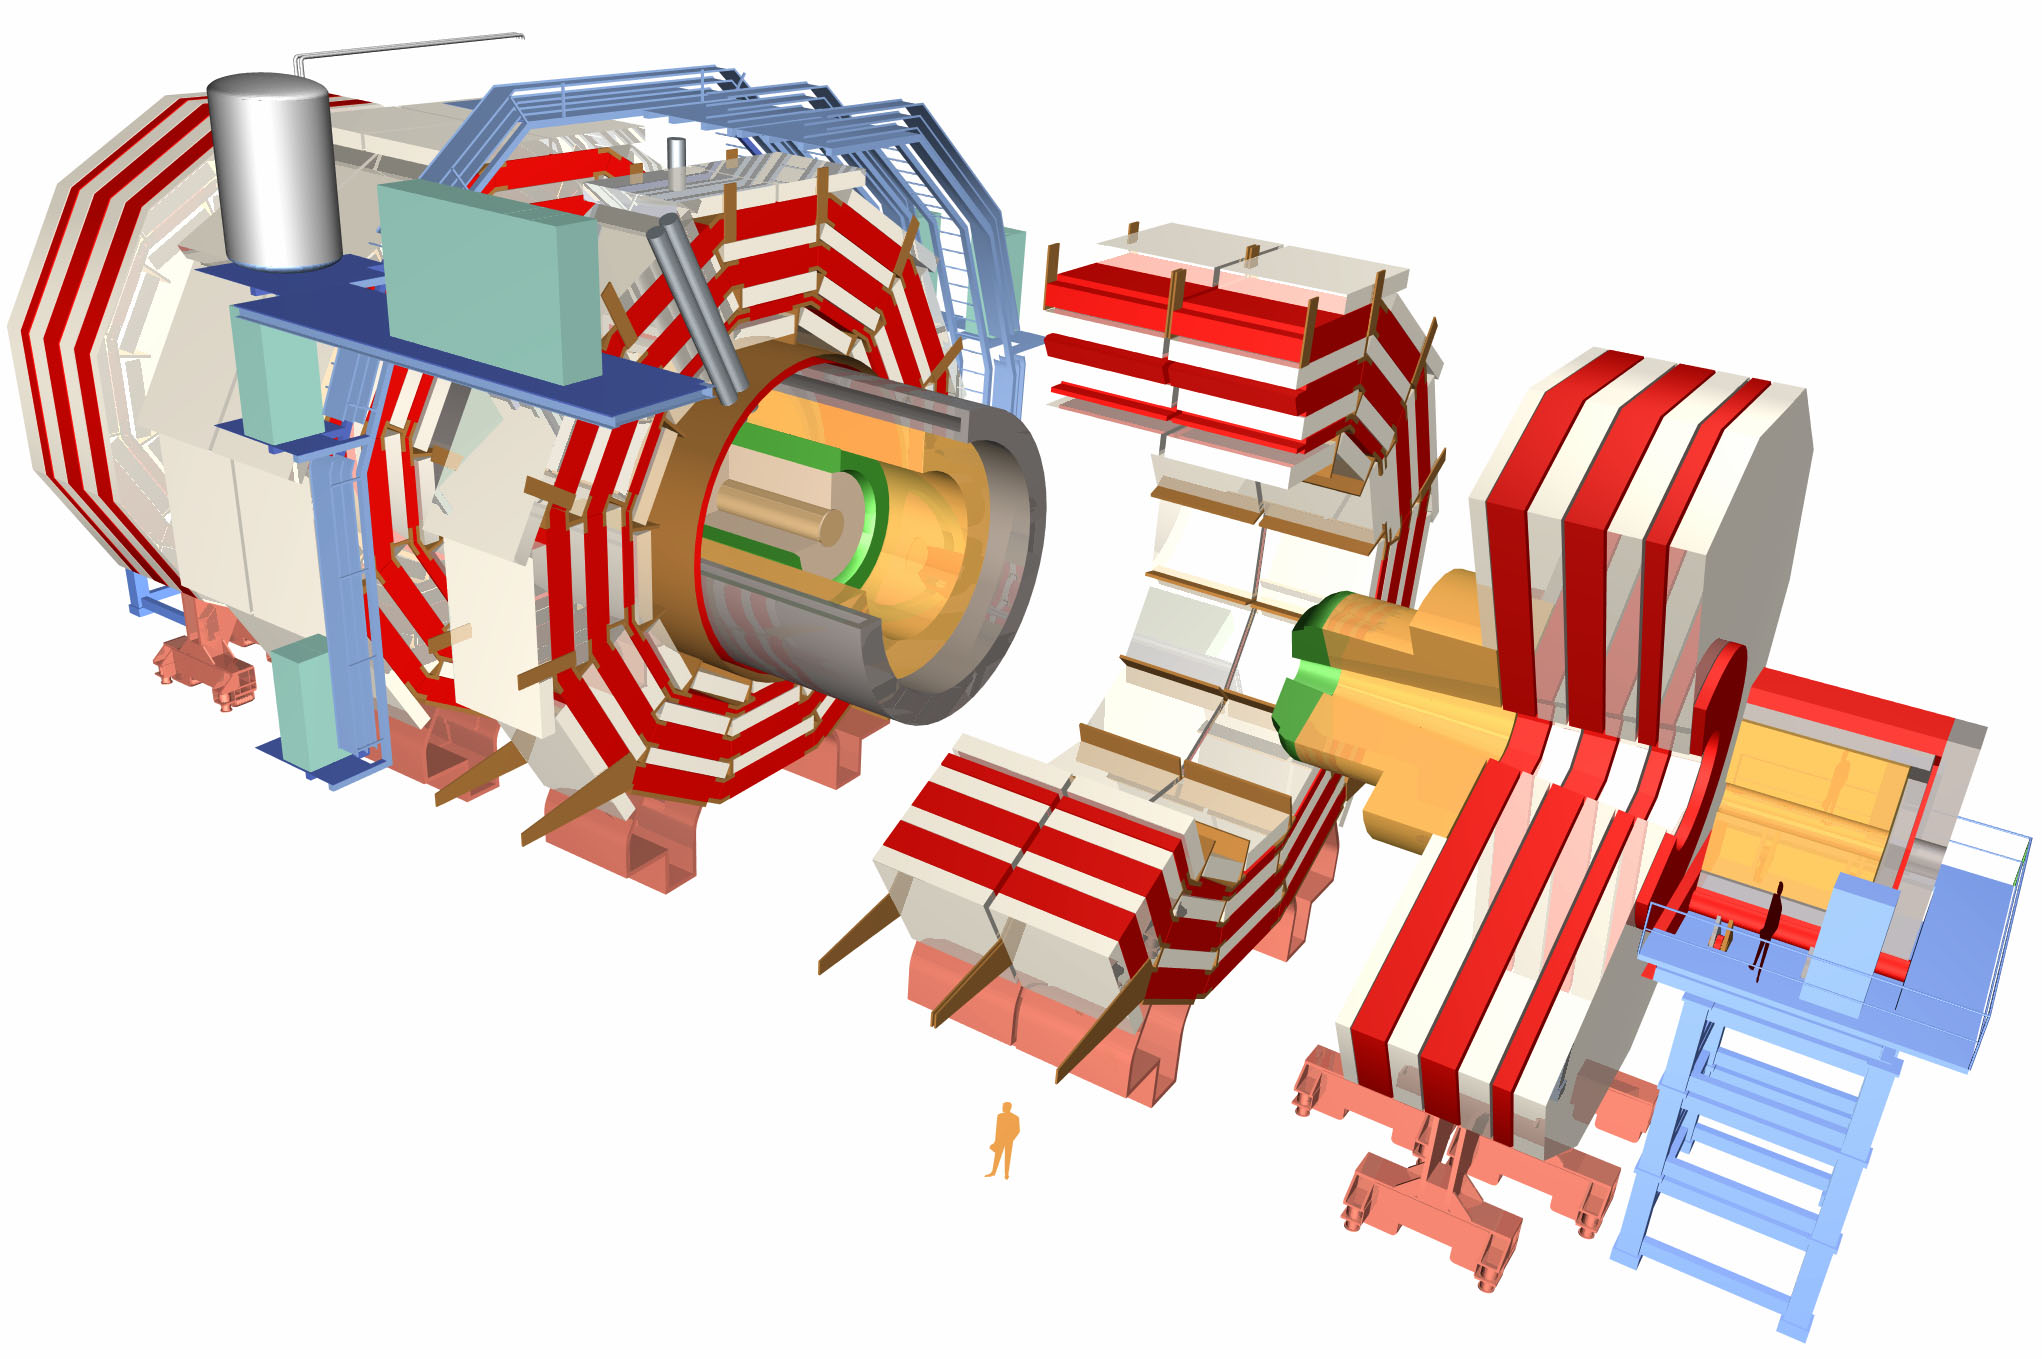
\includegraphics[width=6in]{figures/cms.jpg}
\caption{Deconstructed view of the CMS subdetectors, with human figure for scale. From inside to out, the colored segments correspond to the following systems: light brown is the pixel tracker, cream is the strip tracker, green is the EM calorimeter, orange is the hadronic calorimeter, grey is the solenoid, red is the yoke with white muon chambers \cite{1748-0221-3-08-S08004}. }
\label{fig:cms}
\end{figure}

\subsection{Tracking detectors}

The inner tracking detectors of CMS is supported by a 5.30 m long tube with an inner diameter of 2.38 m suspended from the HCAL barrel. The trackers contain 1,440 pixel and 15,148 strip detector modules, composing the pixel detector and silicon strip tracker, respectively. The detectors are responsible for measuring the trajectories of charged particles, essential to measuring the momenta of particles with energy $>$ 1 $\GeV$ in the range $|\eta|<2.5$, and to reconstructing secondary vertices and impact parameters, needed to identify heavy flavor particles. Being closest to the beam interaction point (IP), the tracking detectors are subjected to the highest radiation doses, and their material may interfere with the trajectories of primary particles through multiple scattering, bremsstrahlung, photon conversion, or nuclear interactions, necessitating the use of silicon technology. Additionally, due to the high particle flux of around 1,000 particles per 25 ns bunch crossing, the detectors must have both high granularity to resolve the trajectories of particles reliably and fast readout times to reduce occupancy from high flux and pileup conditions. 

\indent The detector modules of the tracking detector are shown schematically in Figure~\ref{fig:tracker}. The innermost section, labeled PIXEL, is the pixel detector, composed of 66 million 100 $\mu$m $\times$ 150 $\mu$m pixels on modules layered in three barrels at radii 4.4, 7.3, and 10.2 cm and two disks on each end at $z = \pm34.5, \pm46.5$ cm. A deconstructed barrel pixel module is shown in Figure~\ref{fig:pixmodule}, with the sensor bump-bonded onto readout chips (ROCs) controlled and powered by high-density interconnect (HDI) boards. When a charged particle passes through a pixel sensor, consisting of $n$-type pixels implanted on a high-resistance $n$-type substrate, charge carriers are induced in the conduction band of the substrate. These charge carriers then drift in the 4 T magnetic field to the nearby pixels, where an analog signal is read out, amplified, and digitized by the ROC. This drift is called charge sharing. The end cap pixel modules have a similar construction but with different pixel sensor geometries, called plaquettes. The pixel detector has a resolution of $10-40$ $\mu$m, sufficient for the imposed design requirements. 

\begin{figure}[tbh]
\centering
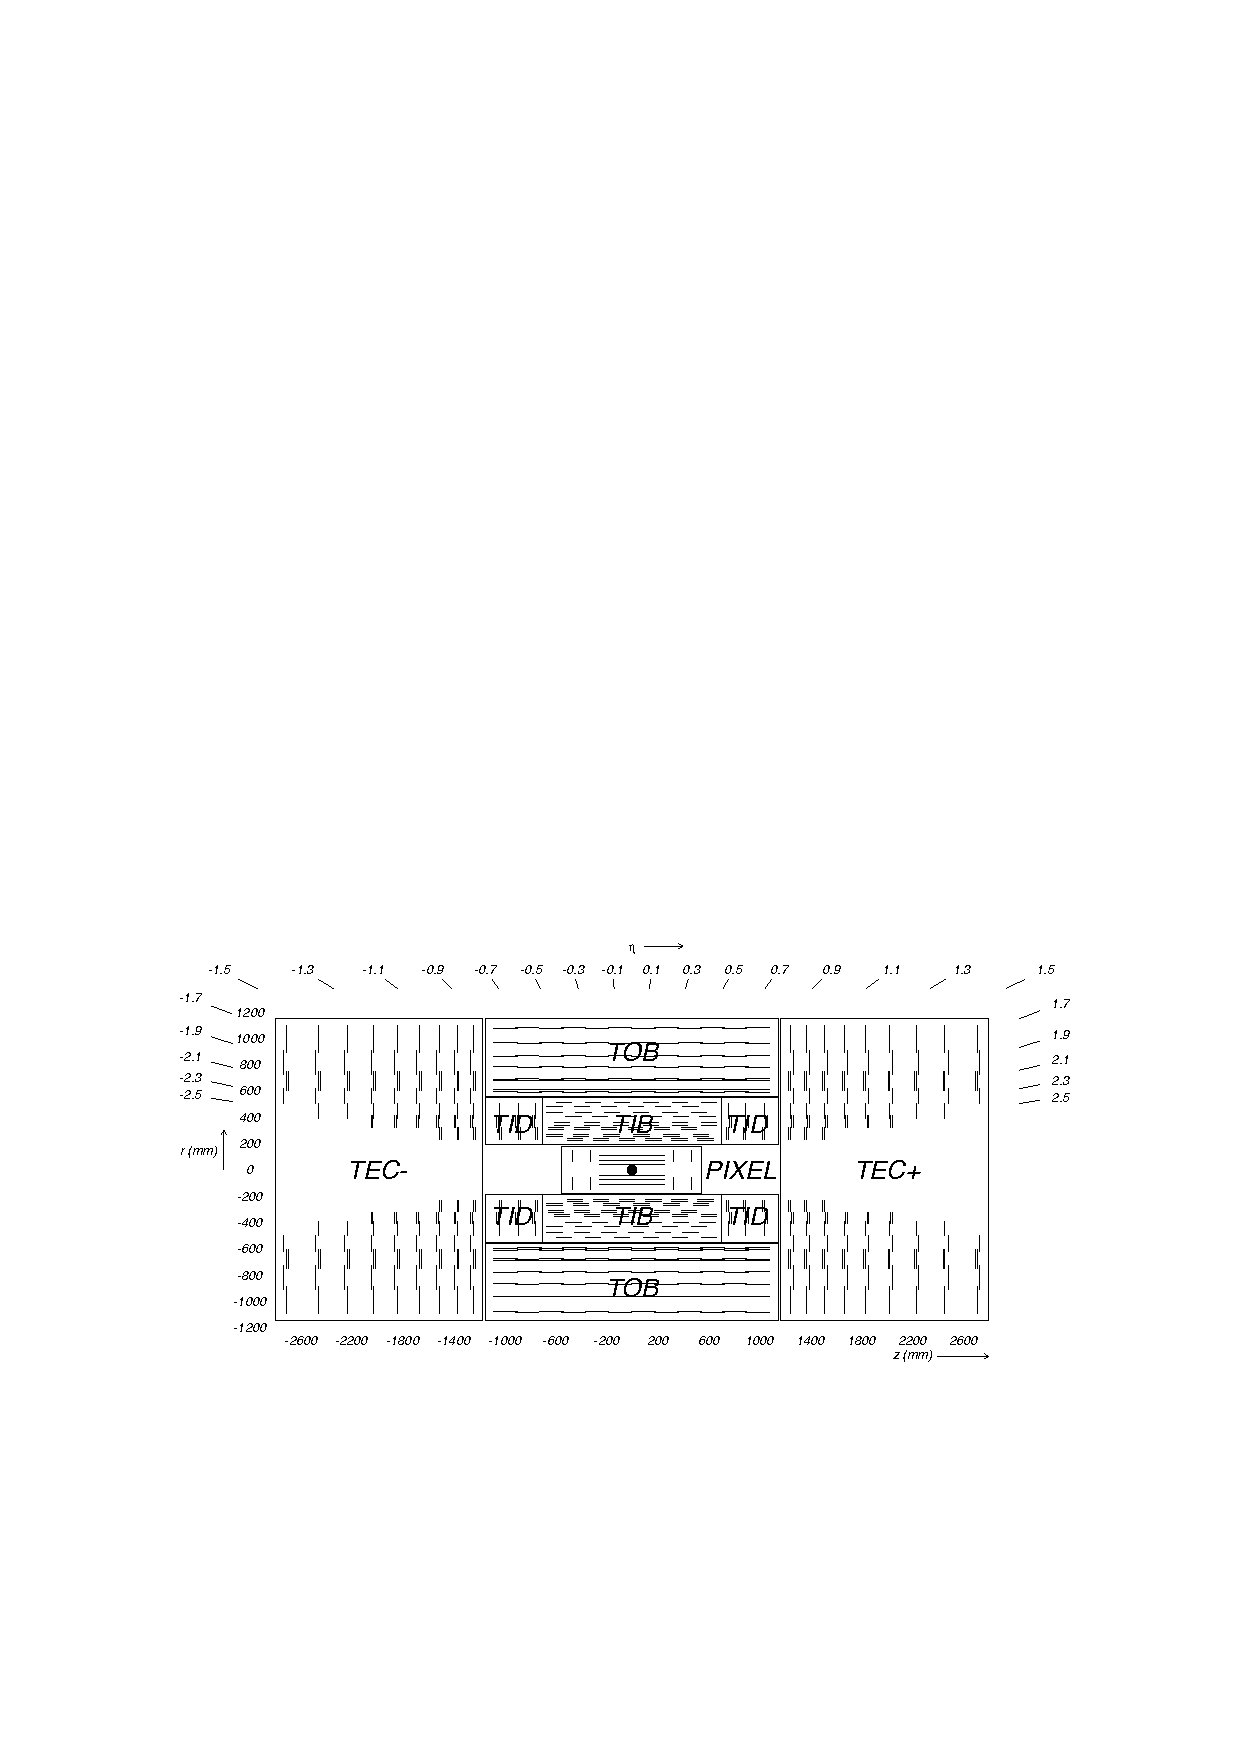
\includegraphics[width=6.5in]{figures/tracker.pdf}
\caption{Schematic diagram of tracking detectors with radial distance of modules, shown as black lines, from center on the left axis, $z$-dimension on the bottom axis, and $\eta$ accross the top \cite{1748-0221-3-08-S08004}.}
\label{fig:tracker}
\end{figure}

\begin{figure}[tbh]
\centering
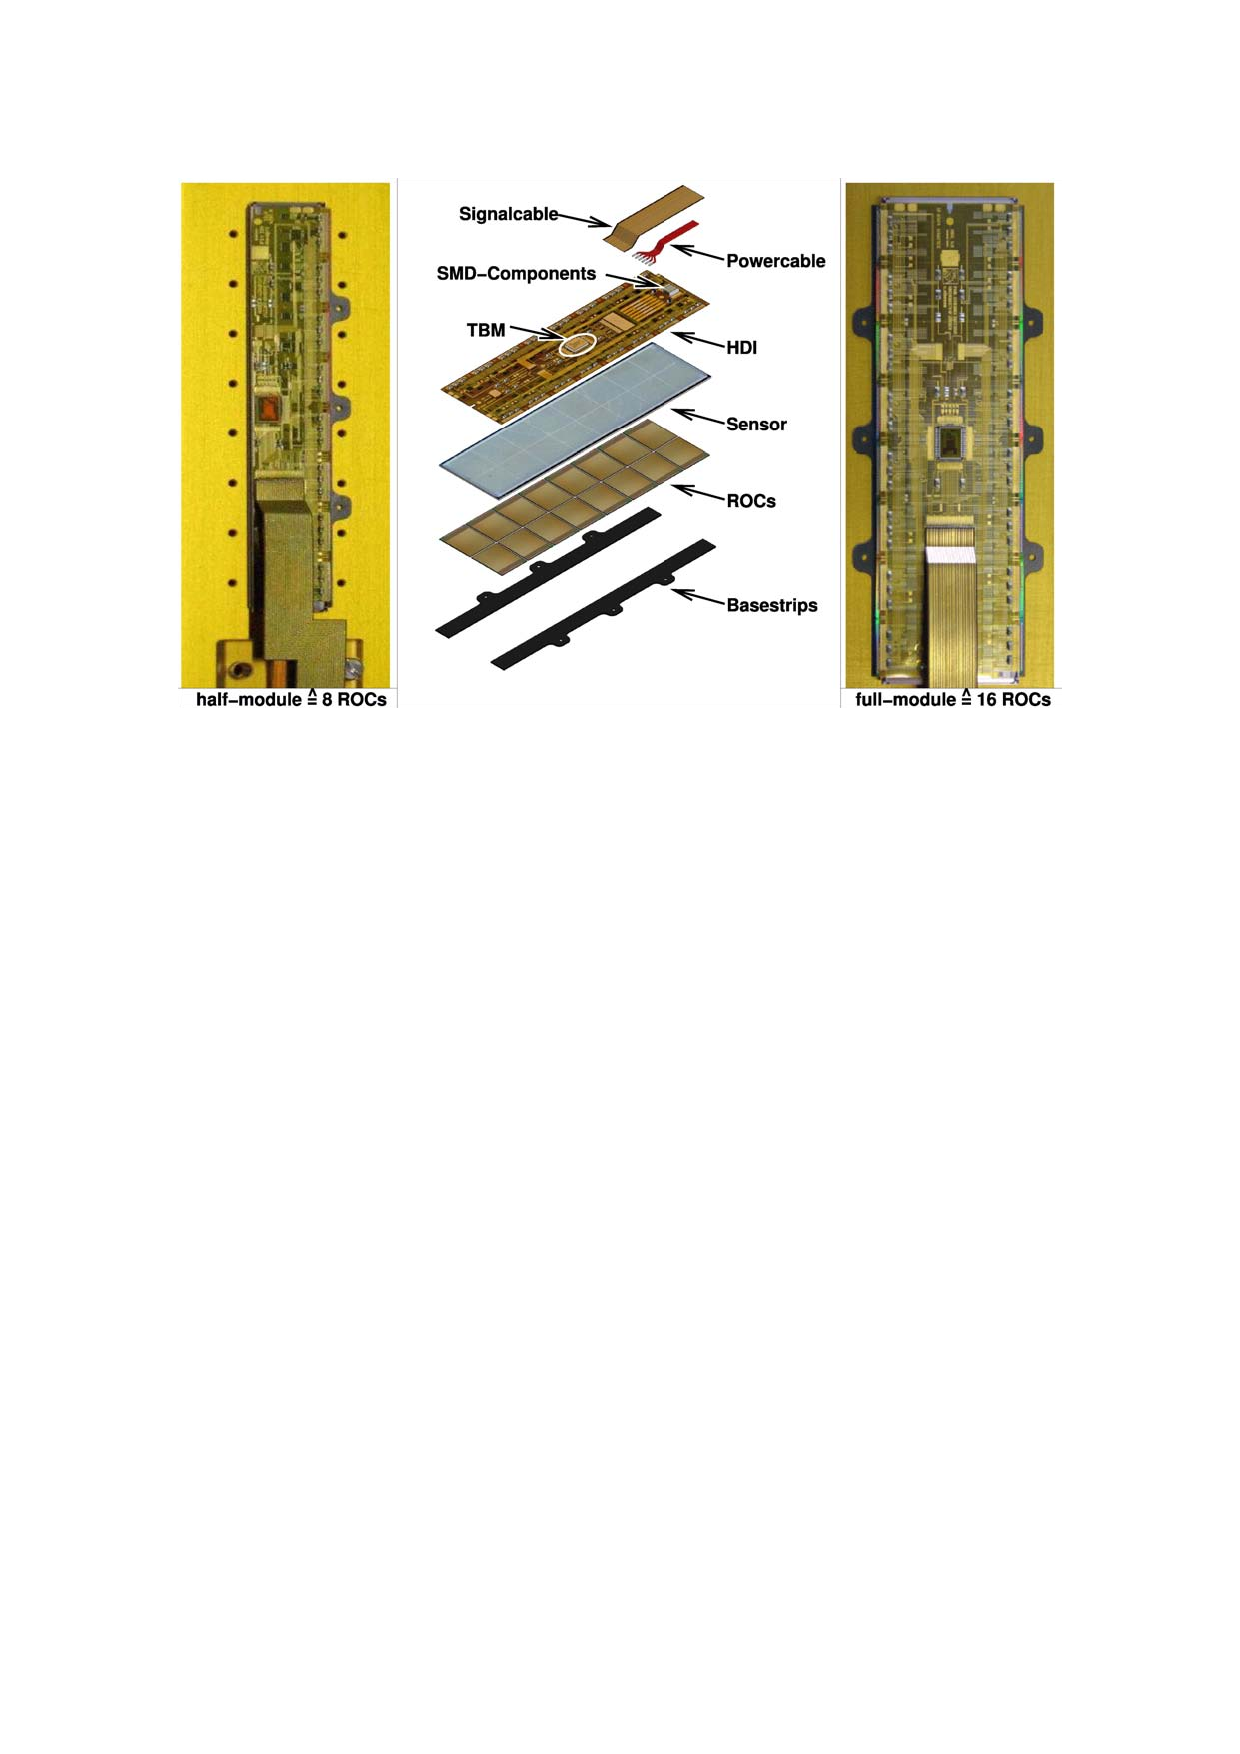
\includegraphics[width=5.5in]{figures/pixelmodule.pdf}
\caption{Deconstructed barrel pixel module showing module components \cite{1748-0221-3-08-S08004}.}
\label{fig:pixmodule}
\end{figure}

\indent The remaining modules of the tracking detector form the strip tracker, which fills the volume between $20-116$ cm radially, and $118$ cm in $z$. These 15,148 modules are divided into the following sections: tracker inner barrel (TIB), with four layers, tracker outer barrel (TOB) with six layers, tracker inner disks (TID) with six layers, and tracker end caps (TEC) with nine layers. The average particle occupancy at distances greater than $20$ cm from the IP is low enough compared to regions closer to the beam line that the strip tracker is not required to have the same granularity as the pixel detector, thus, twenty nine different strip module designs, of different sizes and orientations, are used. The physical principles behind the strip tracker are the same as the pixel detector: charged particles liberate conduction band electrons, which drift toward readout sensors. To enhance the effect of the charge carriers' drift in the magnetic field, the strip detectors are tilted, yielding a resolution of approximately 30 $\mu$m. Excluding defective modules, the detection efficiency of the strip tracker is nearly 100\% (Figure~\ref{fig:stripeff}) \cite{Chatrchyan:2014fea}.

\begin{figure}[tbh]
\centering
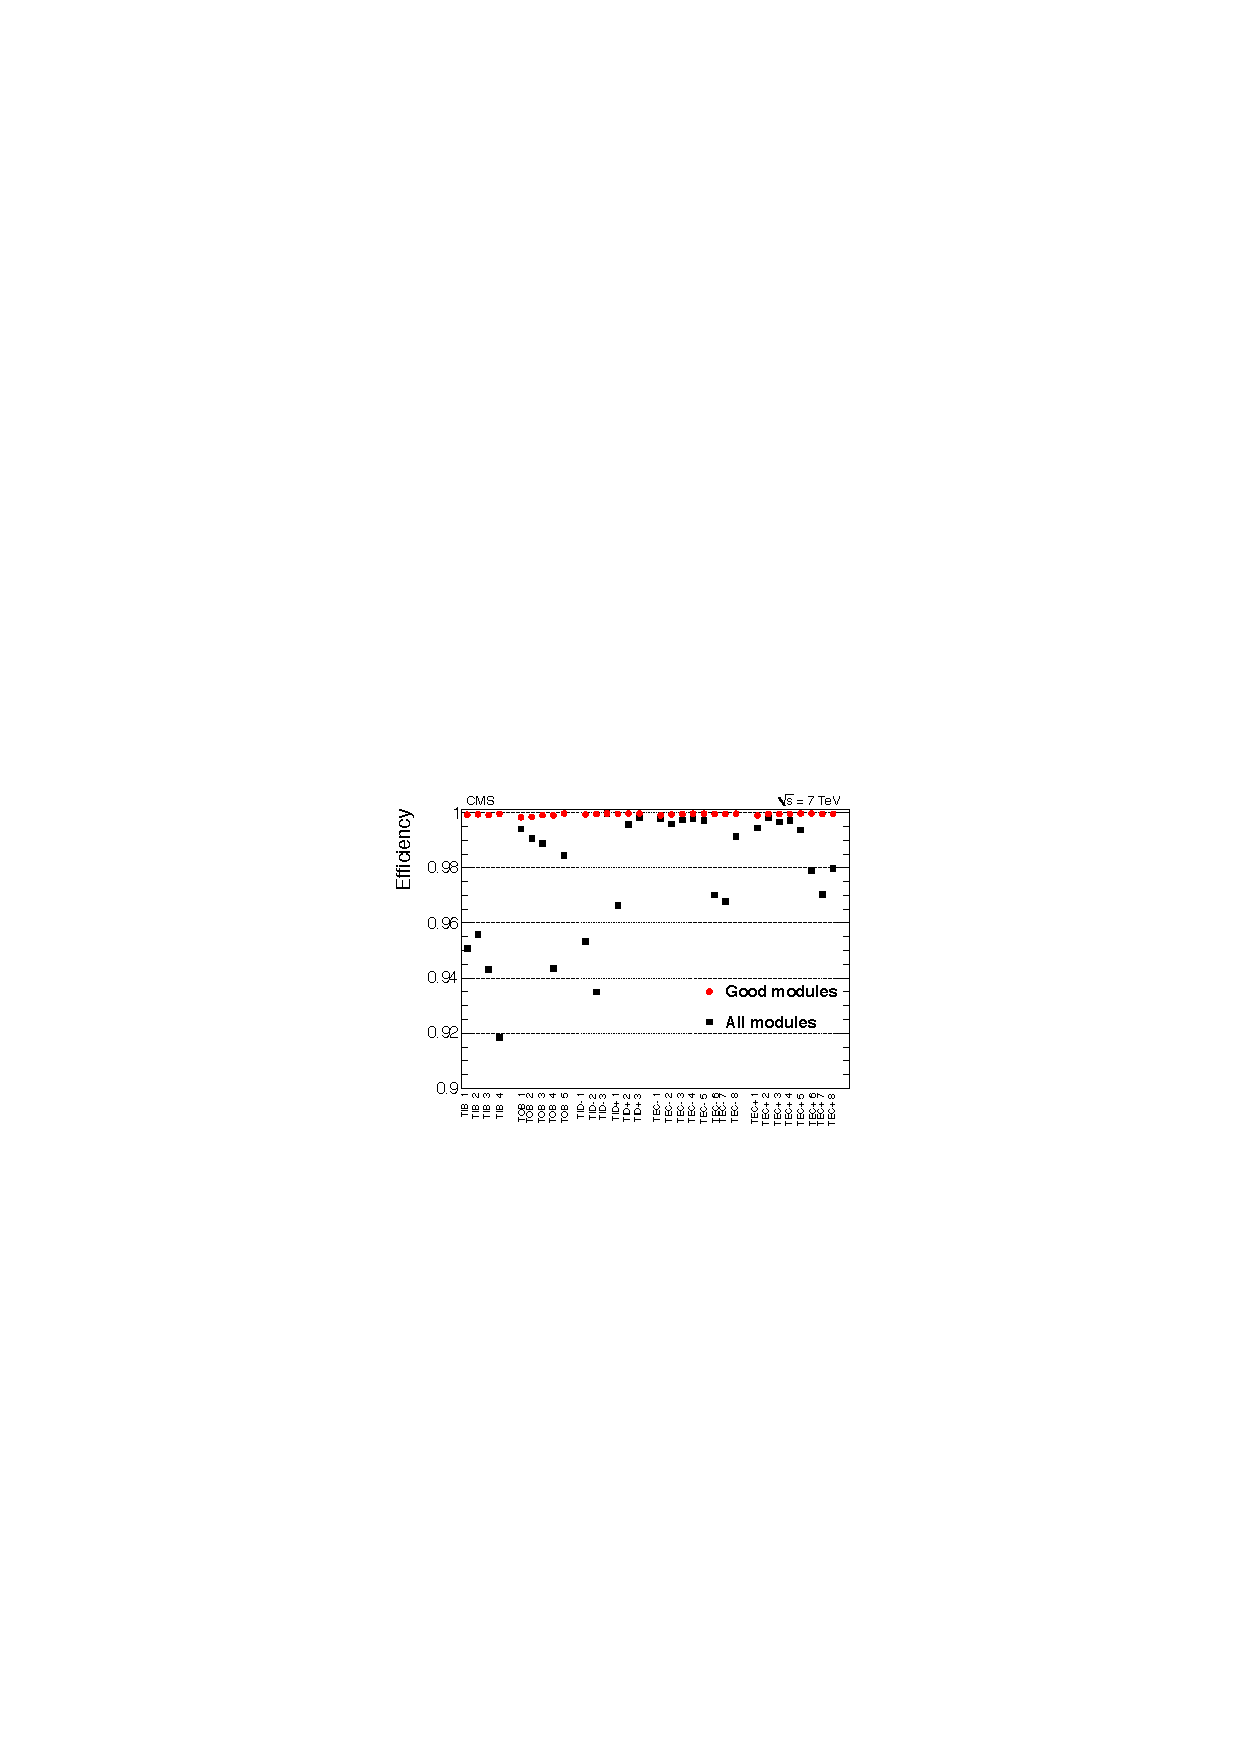
\includegraphics[width=5in]{figures/stripeff.pdf}
\caption{Average hit efficiencies of the strip tracker layers \cite{1748-0221-3-08-S08004}.}
\label{fig:stripeff}
\end{figure}

\subsection{Electromagnetic calorimeter}

The electromagnetic calorimeter (ECAL) consists of 61,200 lead tungstate crystal modules in the ECAL barrel (EB) region, covering $|\eta|<1.479$, and 7,324 modules in each ECAL end cap (EE), covering $1.479<|\eta|<3$. The crystals are oriented radially, as shown in Figure~\ref{fig:ecal}, at angles around three degrees in the EB and two to eight degrees in the EE from the vector to the IP to avoid cracks where particles could escape. The various supercrystal geometries are combined to form supermodules in the EB and two D-electrodes (Dees) on each end cap. The front faces of the EB crystals are at $r=1.29$ m, and present a cross section around $22$ mm$\times$$22$ mm. The EB extends to an outer radius of 1.77 m. The end cap envelopes are at $\pm315.4$ cm relative to the IP in $z$. The crystals themselves have a truncated pyramidal shape. Except for one face on the EB crystals that is depolished to account for nonuniformity in light production from the crystal shape, the crystals are polished on all sides to increase internal reflection. 

\indent The ECAL is responsible for recovering the energy of electrons and photons from the showers of scintillation light produced in the crystals. The accuracy of this measurement is of particular importance in the design of CMS, since the Higgs decay to photons and leptons are key channels in the Higgs search, one of the primary purposes of CMS. In front of each set of endcap crystals, the ECAL contains preshower detectors, consisting of a thin layer of lead followed by a thin layer of silicon strip sensors to create and detect showers from minimum ionizing particles. The primary purpose of the preshower detectors is to identify and veto neutral pion production, in addition to improving the overall position resolution of the ECAL.

\begin{figure}[tbh]
\centering
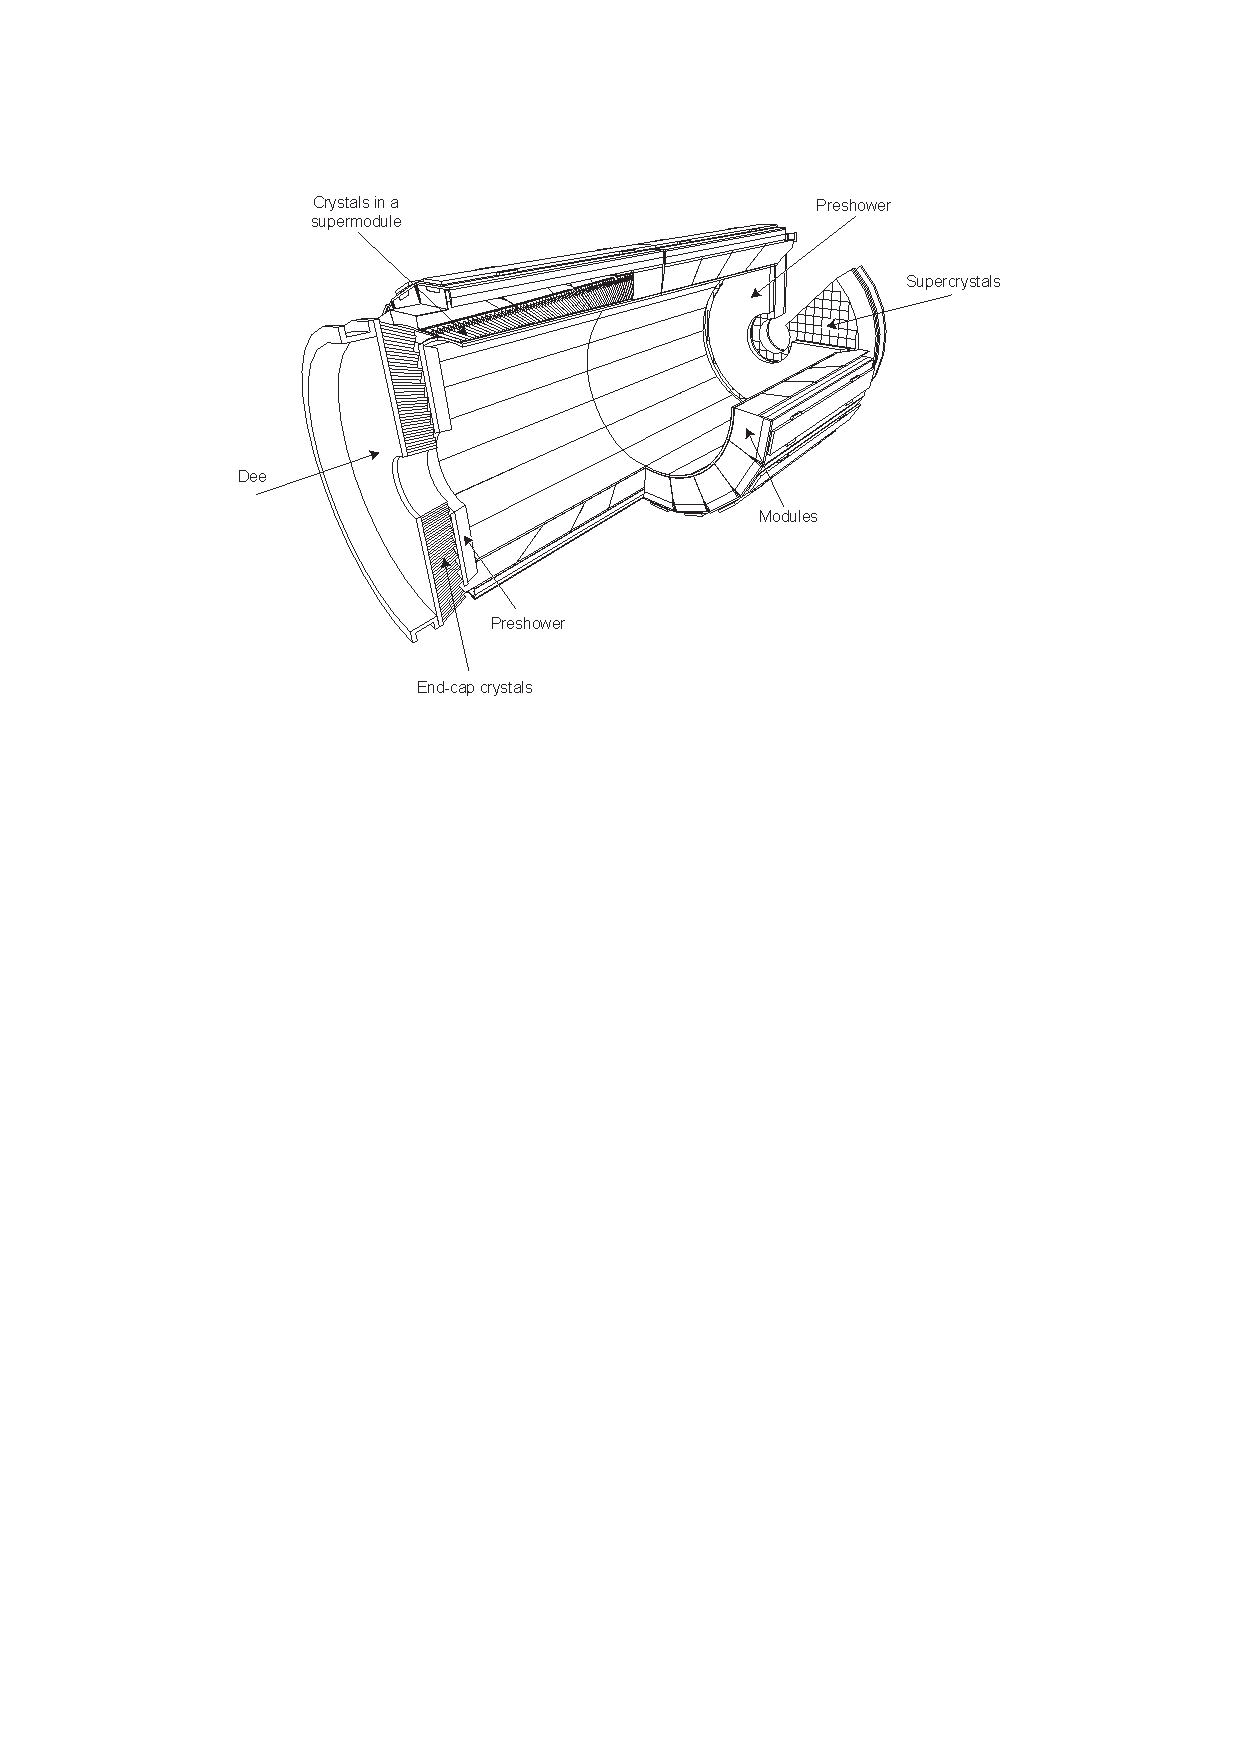
\includegraphics[width=5in]{figures/ecal.pdf}
\caption{Schematic layout of the ECAL crystal modules \cite{1748-0221-3-08-S08004}.}
\label{fig:ecal}
\end{figure}

\indent Lead tungstate crystals were chosen for the construction of the ECAL because of their radiation hardness. The following properties enable a compact detector with sufficiently high granularity: a high density of 8.28 g/$\rm{cm}^3$, a short radiation length of 0.89 cm, and a small Moliere radius of 2.2 cm. Additionally, the crystals have a fast scintillation decay time of about 25 ns, the same time between bunch crossings, enabling fast response and read out. At operating temperature, about 4.5 photoelectrons are collected in the attached photodetectors per $\MeV$ of incident particle energy from the blue-green scintillation light produced in the crystals. EB crystals are glued to avalanche photodiodes (APDs) while EE crystals are read by vacuum phototriodes (VPTs), each specially designed for the CMS ECAL, as shown in Figure~\ref{fig:crystalmodules}. 

\begin{figure}[tbh]
\centering
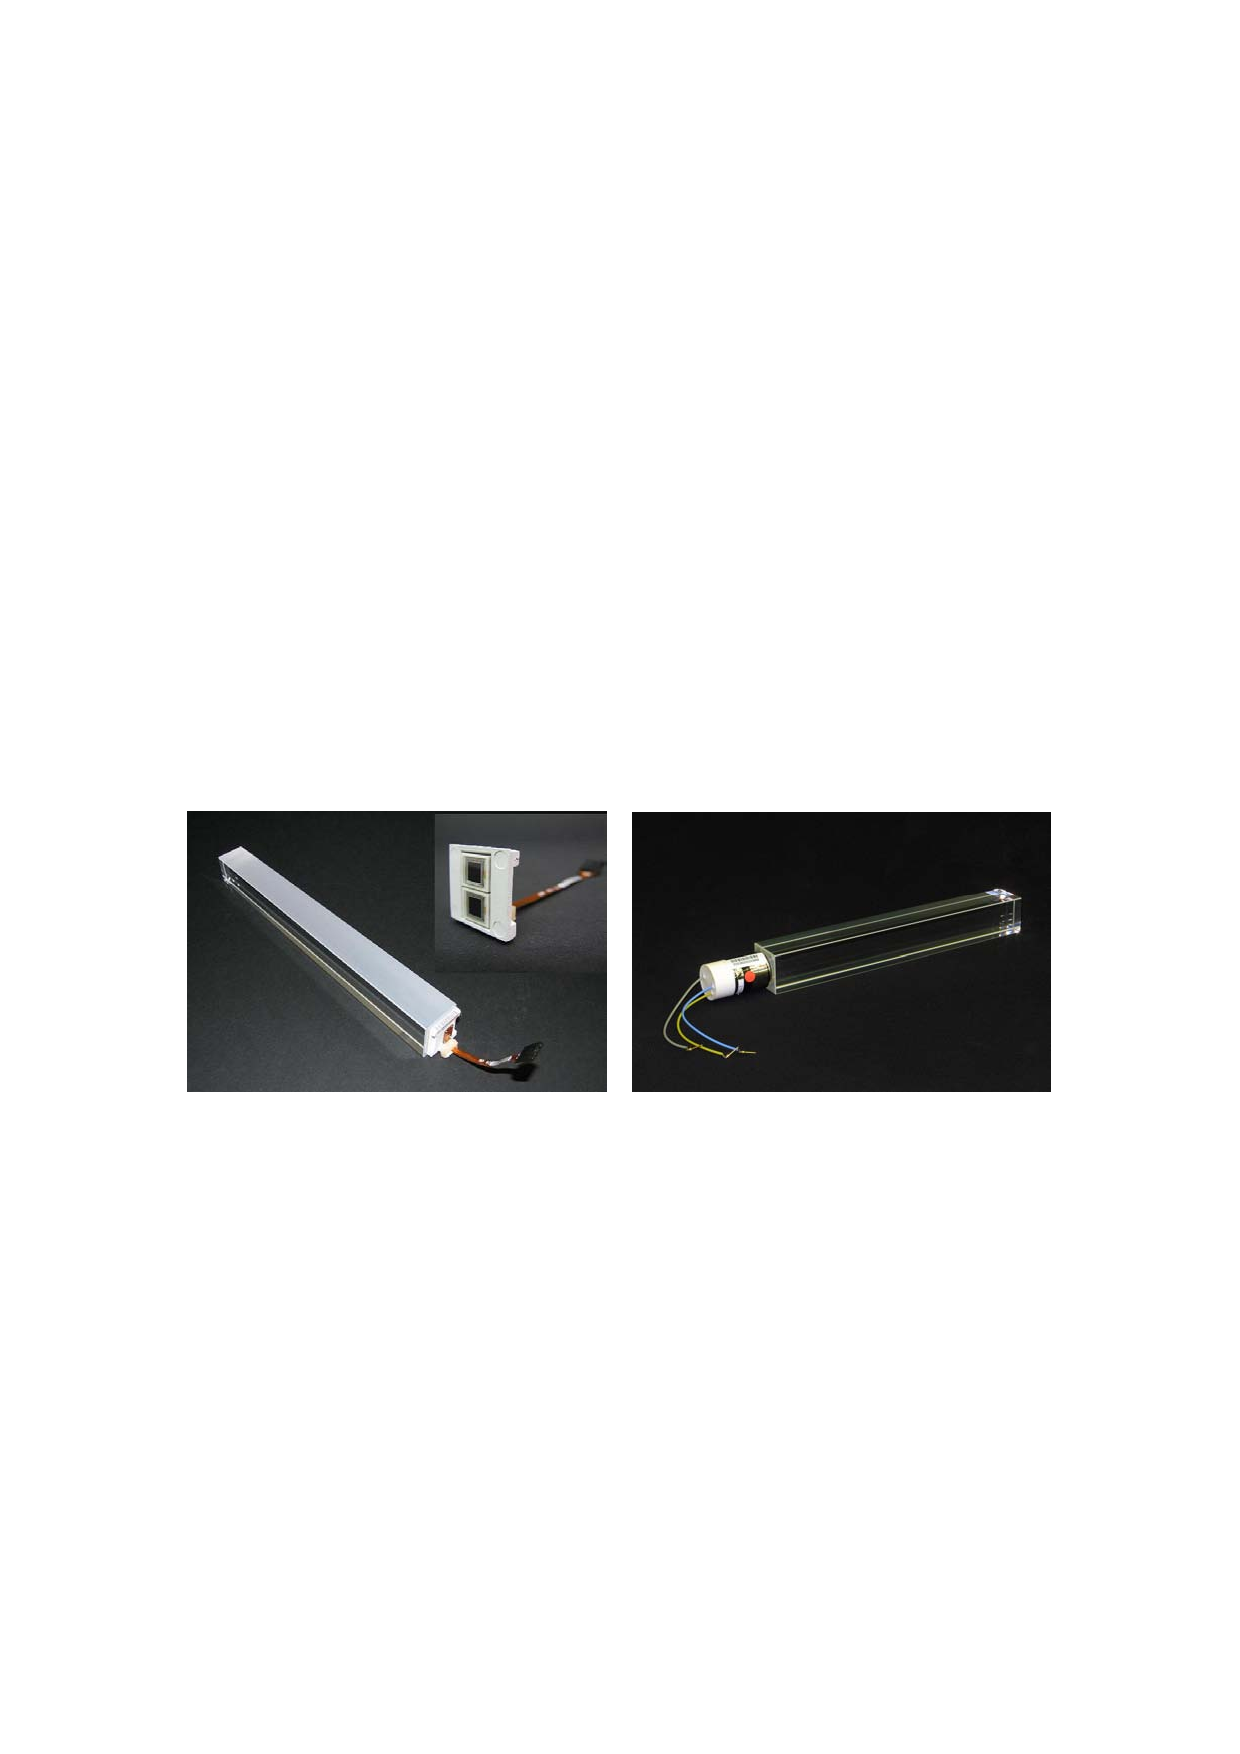
\includegraphics[width=6in]{figures/crystalmodules.pdf}
\caption{ECAL barrel crystal with one depolished face attached to avalanche photodiode photodetector (left) and ECAL end cap crystal attached to vacuum phototriode (right) \cite{1748-0221-3-08-S08004}.}
\label{fig:crystalmodules}
\end{figure}

\indent The energy resolution of the ECAL depends on the energy of the incident particle, and can be parametrized as the sum of three terms:
\begin{equation}
\bigg(\frac{\sigma}{E}\bigg)^2 = \bigg(\frac{S}{\sqrt{E}}\bigg)^2 + \bigg(\frac{N}{E}\bigg)^2 + C^2
\end{equation}
The first term, called the stochastic term, arises from fluctuations in the lateral shower containment, photostatistics, and fluctuations in energy deposited in the preshower detector. The second term, called the noise term, arises from electronic, digitization, and pileup noise. The third term, called the constant term, arises from nonuniformity in light collection, calibration errors, and leakage from the back of the crystals. Test beam experiments using electron beams with momenta $20-250$ $\GeV$ found approximate values for the parameters: $S=0.028$, $N=0.12$, and $C=0.003$. 

\subsection{Hadronic calorimeter}

The hadronic calorimeter (HCAL) lies primarily within the bore of the CMS solenoid, surrounding the ECAL, between 1.77 m and 2.95 m from the beam line, covering up to $|\eta|<5.2$. The HCAL is divided into four subsystems, shown schematically in Figure~\ref{fig:hcal}: the HCAL barrel (HB) region, covering $|\eta|<1.3$, the HCAL end caps (HE), covering $1.3<|\eta|<3$, the HVAL outer (HO) calorimeter, or tail catcher, double covering the EB and HB regions to ensure complete shower absorption, outside the solenoid, and the HCAL forward (HF) calorimeter, covering up to $|\eta|<5.2$ at 11.2 m from the IP. The primary function of the HCAL is to measure the energy and direction of hadronic jets, showers of particles produced from particles composed of quarks and gluons interacting with the detector material. Another important function of the HCAL is to contribute to the measurement of MET, which is a key variable in this analysis. 

\begin{figure}[tbh]
\centering
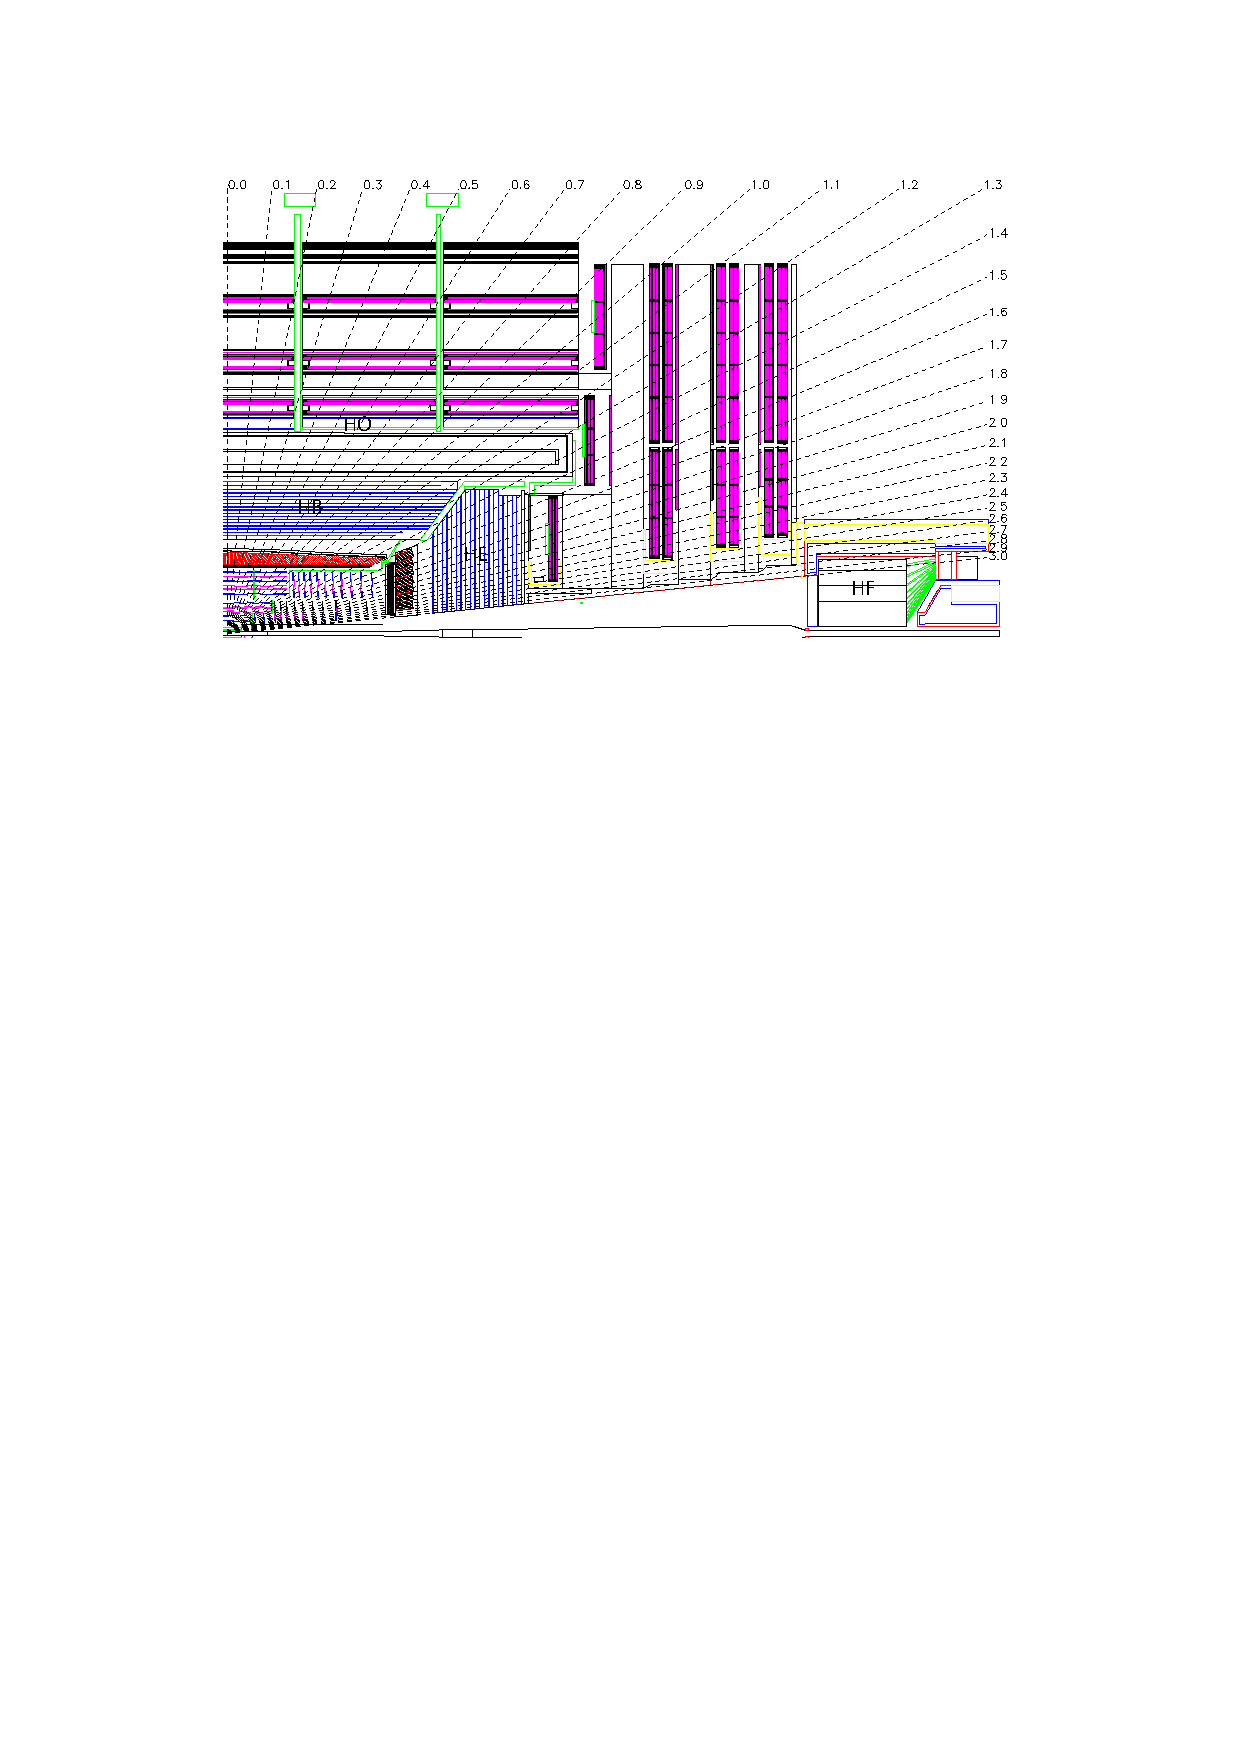
\includegraphics[width=6in]{figures/hcal.pdf}
\caption{Cross sectional view of one quadrant of CMS. The labeled sections are the subsytems of the hadronic calorimeter \cite{1748-0221-3-08-S08004}.}
\label{fig:hcal}
\end{figure}

\indent The HCAL subsystems consist of layers of absorber material and scintillator material. The absorber material causes incident hadrons to shower into quarks and gluons, whose energy is deposited and read out from the scintillator layers. Tiles of scintillator material are organized into units called trays. The HB consists of two half-barrels, each with eighteen identical $\phi$-wedges, each consisting of seventeen layers of scintillator material, with each layer containing 108 trays. The scintillator layers are separated by eight 50.5 mm thick and six 56.5 mm thick brass plates and surrounded by an inner 40 mm thick and outer 75 mm thick steel plate. The HE disks consist of 36 identical $\phi$-wedges, with a total of 1,368 trays of 20,916 trapezoidal scintillator tiles divided into 18 layers, alternating with 79 mm thick brass plates. The HO layers are each divided into 12 $\phi$-sectors, consist of 40 mm thick detector layers of scintillator and aluminum supports, layered into the 75 mm thick steel beams of the return yoke. The HB, HE, and HO tiles are arranged to attain a granularity of $(0.087, 0.087)$ in $(\eta, \phi)$. The scintillation light produced in the HB, HE, and HO tiles is collected by wavelength-shifting (WLS) fibers, grouped by tray in clear fibers leading to optical decoders which arrange the clear fibers into readout towers, transmitted to hybrid photodiodes (HPD) for amplification and readout. The energy resolution of HB+HE versus HB+HE+HO systems for test beam pions is shown in Figure~\ref{fig:eres_hcal}, with a clear improvement when including the HO.

\begin{figure}[tbh]
\centering
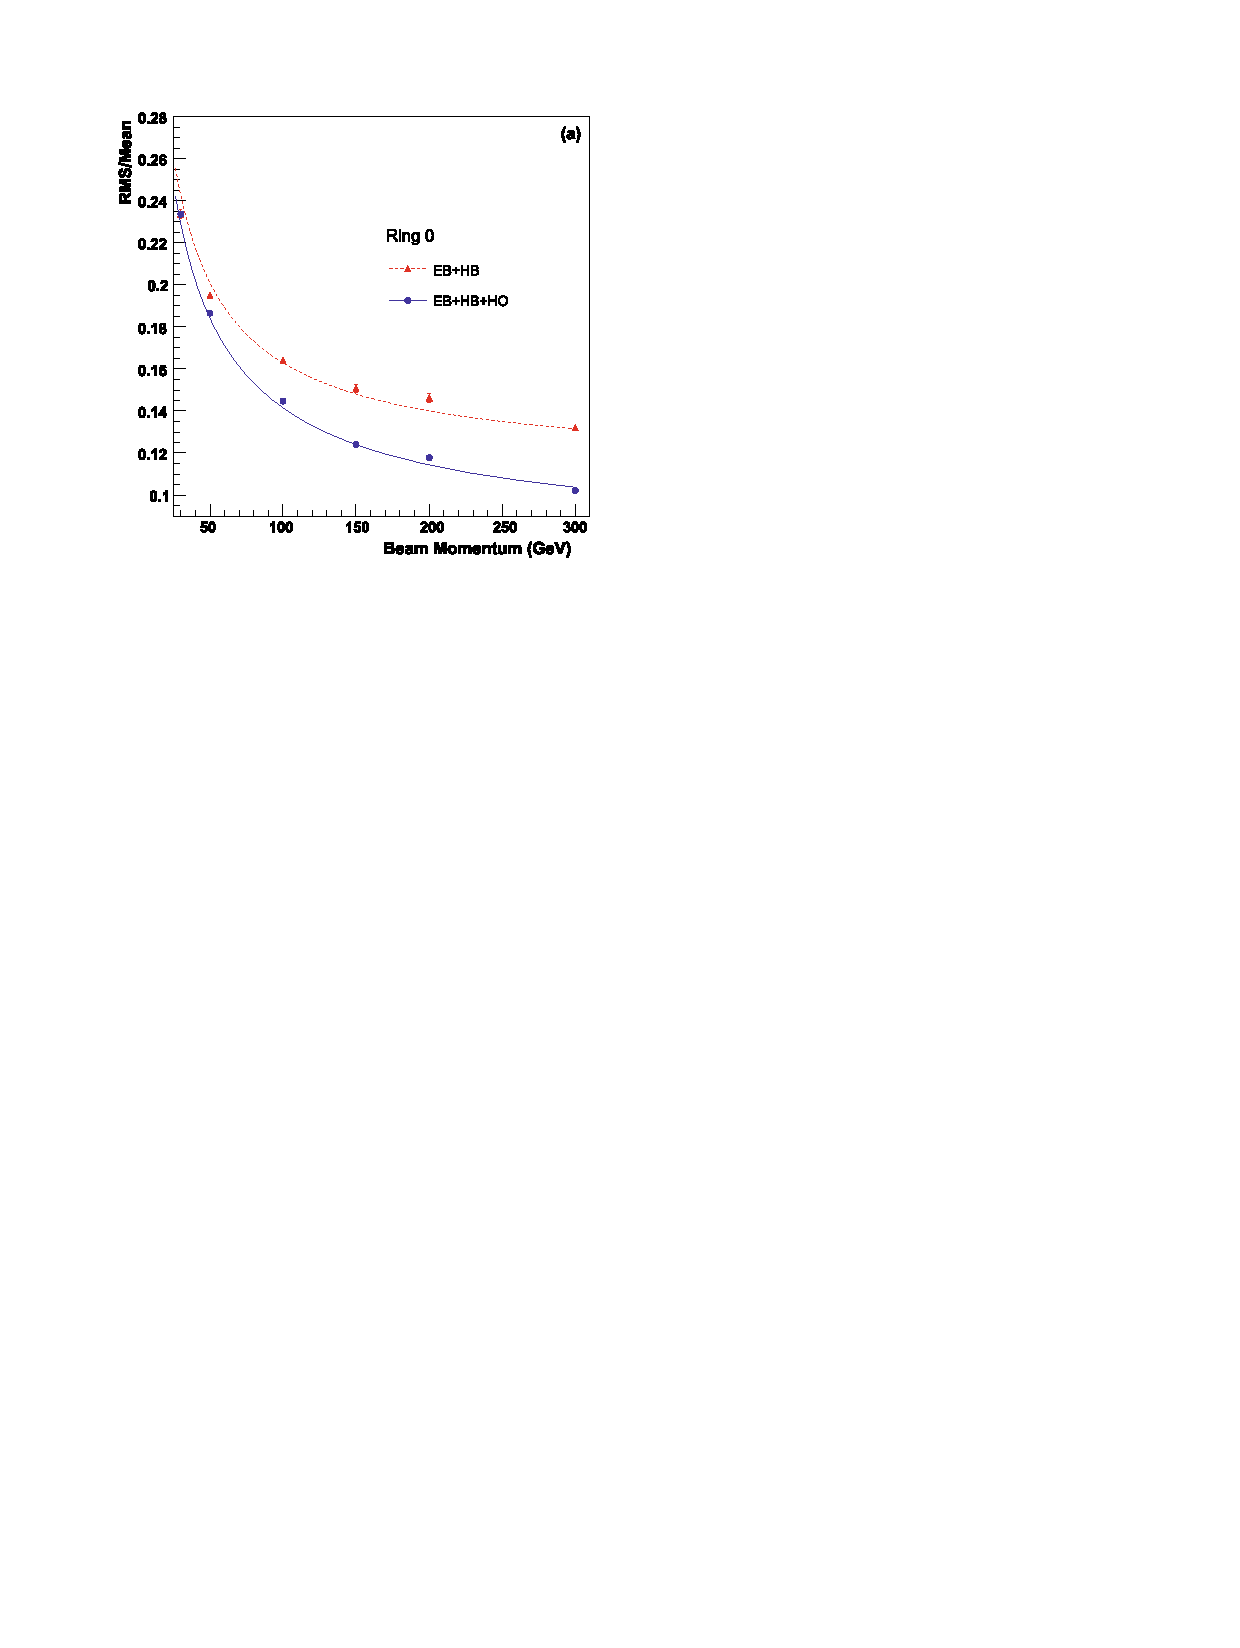
\includegraphics[width=4in]{figures/eres_hcal.pdf}
\caption{Energy resolution of HCAL systems for test beam pions \cite{1748-0221-3-08-S08004}.}
\label{fig:eres_hcal}
\end{figure}

\indent The HF barrels consist of eighteen identical $\phi$-wedges, with layers of 5 mm thick steel plates. Due to higher radiation doses, quartz fibers are used instead of plastic as in the other HCAL subsystems to produce scintillation light. The quartz fibers lie in grooves cut in the steel plates, with half running the full length of the absorber and half starting 22 cm, from the front of the HF barrel. This can be used to classify showers as EM or hadronic, as EM showers deposit most of their energy in the first 22 cm while hadronic showers deposit roughly the same energy throughout the material. Fibers are bundled into towers with a granularity of $(0.175, 0.175)$. Additionally, the HF is used to measure the luminosity of the LHC beam.

\subsection{Muon detectors}

As muons are able to pass through the inner detector material with little radiative losses, the CMS muon system is the outermost subdetector system, consisting of end caps and a barrel region divided into four layers called stations. The barrel region is segmented into regions based on the five 2.536 m yoke rings at $z = 0, \pm5.342, \pm2.686$ and the iron ribs of the yoke support structure. With the goal of reconstructing the momenta and charge of muons over a wide angular and kinematic range, three types of gas-ionization detection mechanisms are employed: drift tubes (DTs), cathode strip chambers (CSCs), and resistive plate chambers (RPCs). 

\indent The barrel DT system consists of drift cells, 13 mm $\times$ 42 mm $\times$ 2.4 m chambers filled with 85\% Ar and 15\% $\rm{CO}_2$ gas, with outer cathode strips and an inner anode wire to read out charge carriers ionized when a charged particle passes through the gas. Four drift cells are stacked, staggered by half a cell, to form superlayers (SLs). SLs are combined in groups of two or three to form drift chambers. The inner three stations have sixty DT chambers, with cells having anode wires running in the $r-\phi$ and z directions. The outer station has seventy DT chambers with cells having anode wires running only in the $r-\phi$ direction. A schematic diagram of the layout of the DT chambers, layered in the iron yoke, is shown in Figure~\ref{fig:DTs}.

\begin{figure}[tbh]
\centering
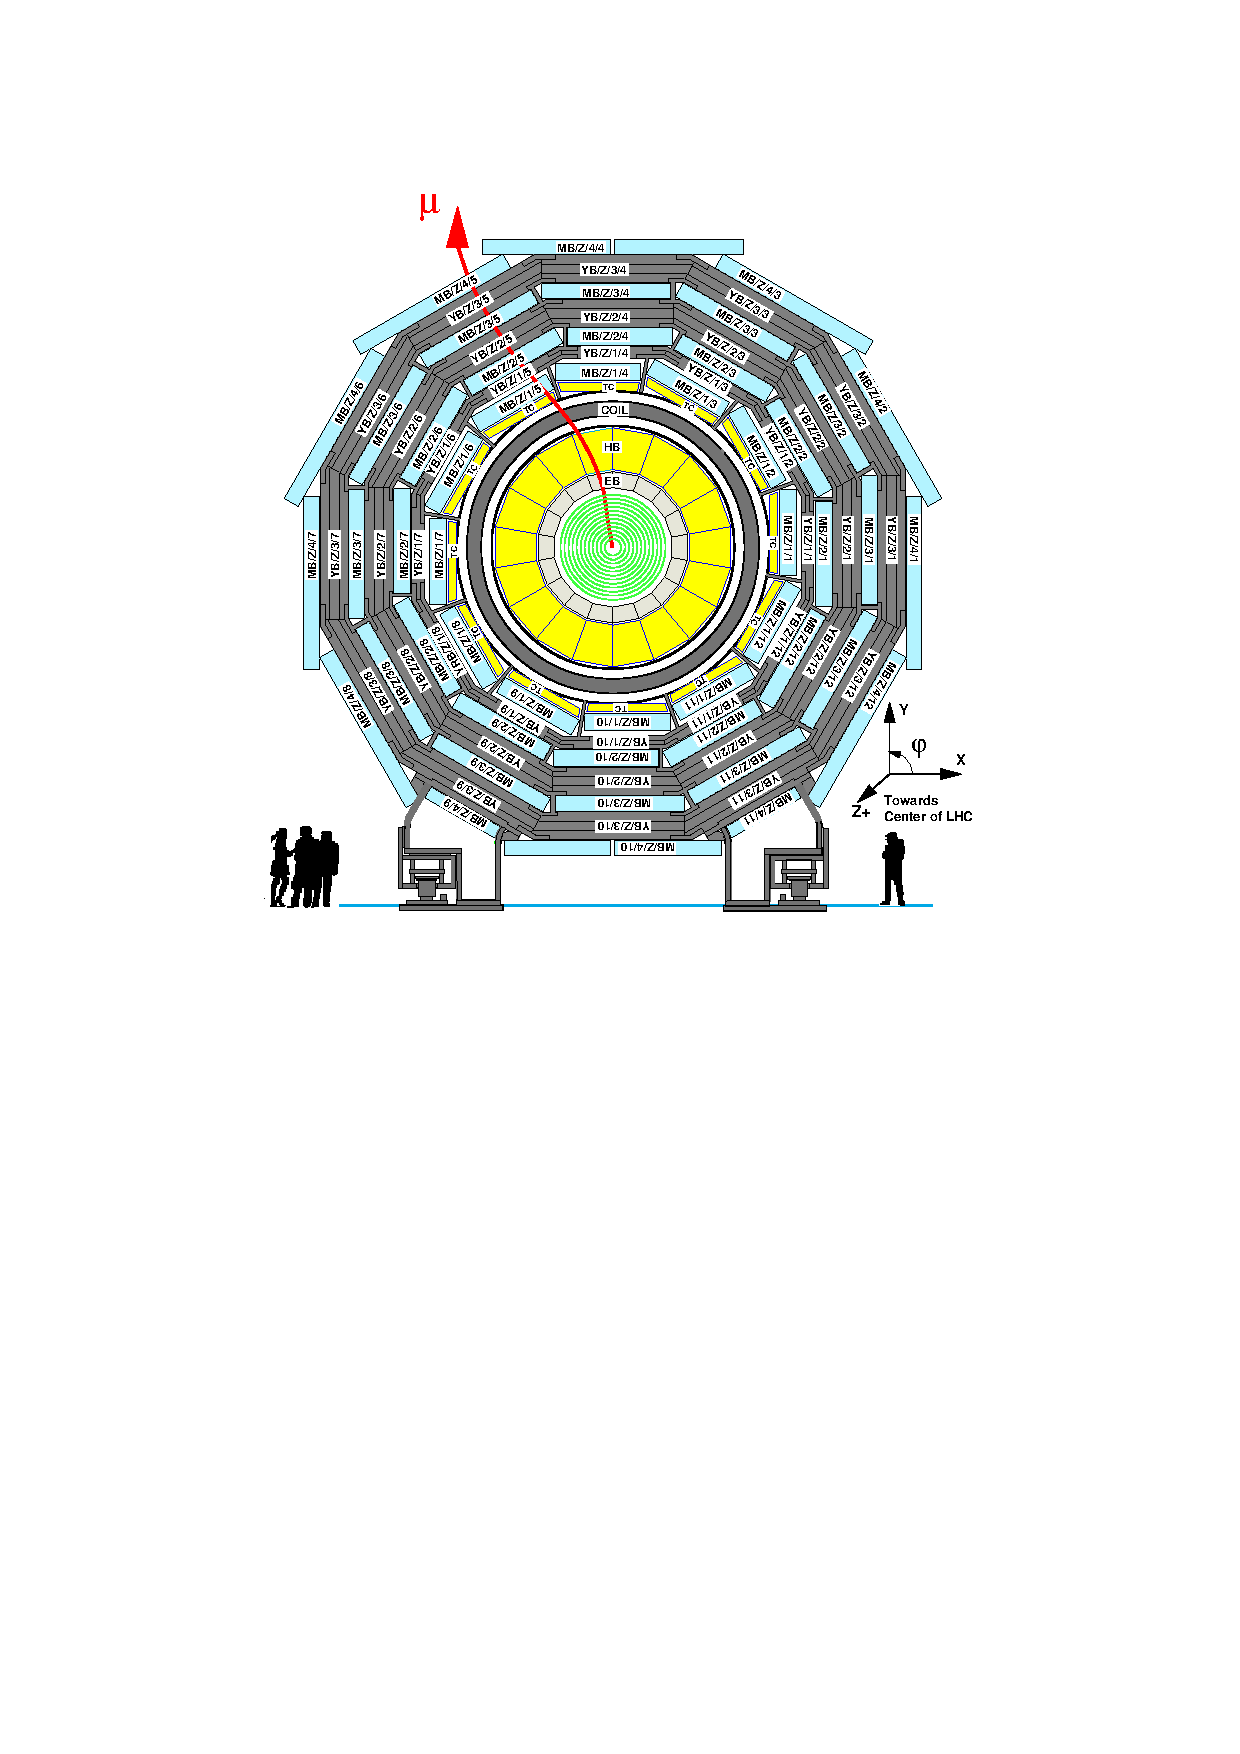
\includegraphics[width=5in]{figures/DTs.pdf}
\caption{Schematic diagram showing DT chambers in light blue \cite{1748-0221-3-08-S08004}.}
\label{fig:DTs}
\end{figure}

\indent The end cap CSC system consists of 468 trapezoidal CSC modules, proportional counters with six azimuthal anode wires running perpendicular to seven radial cathode strips, providing measurements of $r$ and $\phi$ with $80 \mu$m resolution with pseudorapidity coverage $0.9 < |\eta| < 2.4$. Muons passing though the chambers' 40\%:50\%:10\%, Ar:$\rm{CO}_2$:$\rm{CF}_4$ gas mixture produce an avalanche of positively charged carriers, whose signals are interpolated across multiple cathode strips along the anode wires to reconstruct the avalanche position. The position of the CSCs in a cutout quadrant of CMS is shown in Figure~\ref{fig:cscs}.

\begin{figure}[tbh]
\centering
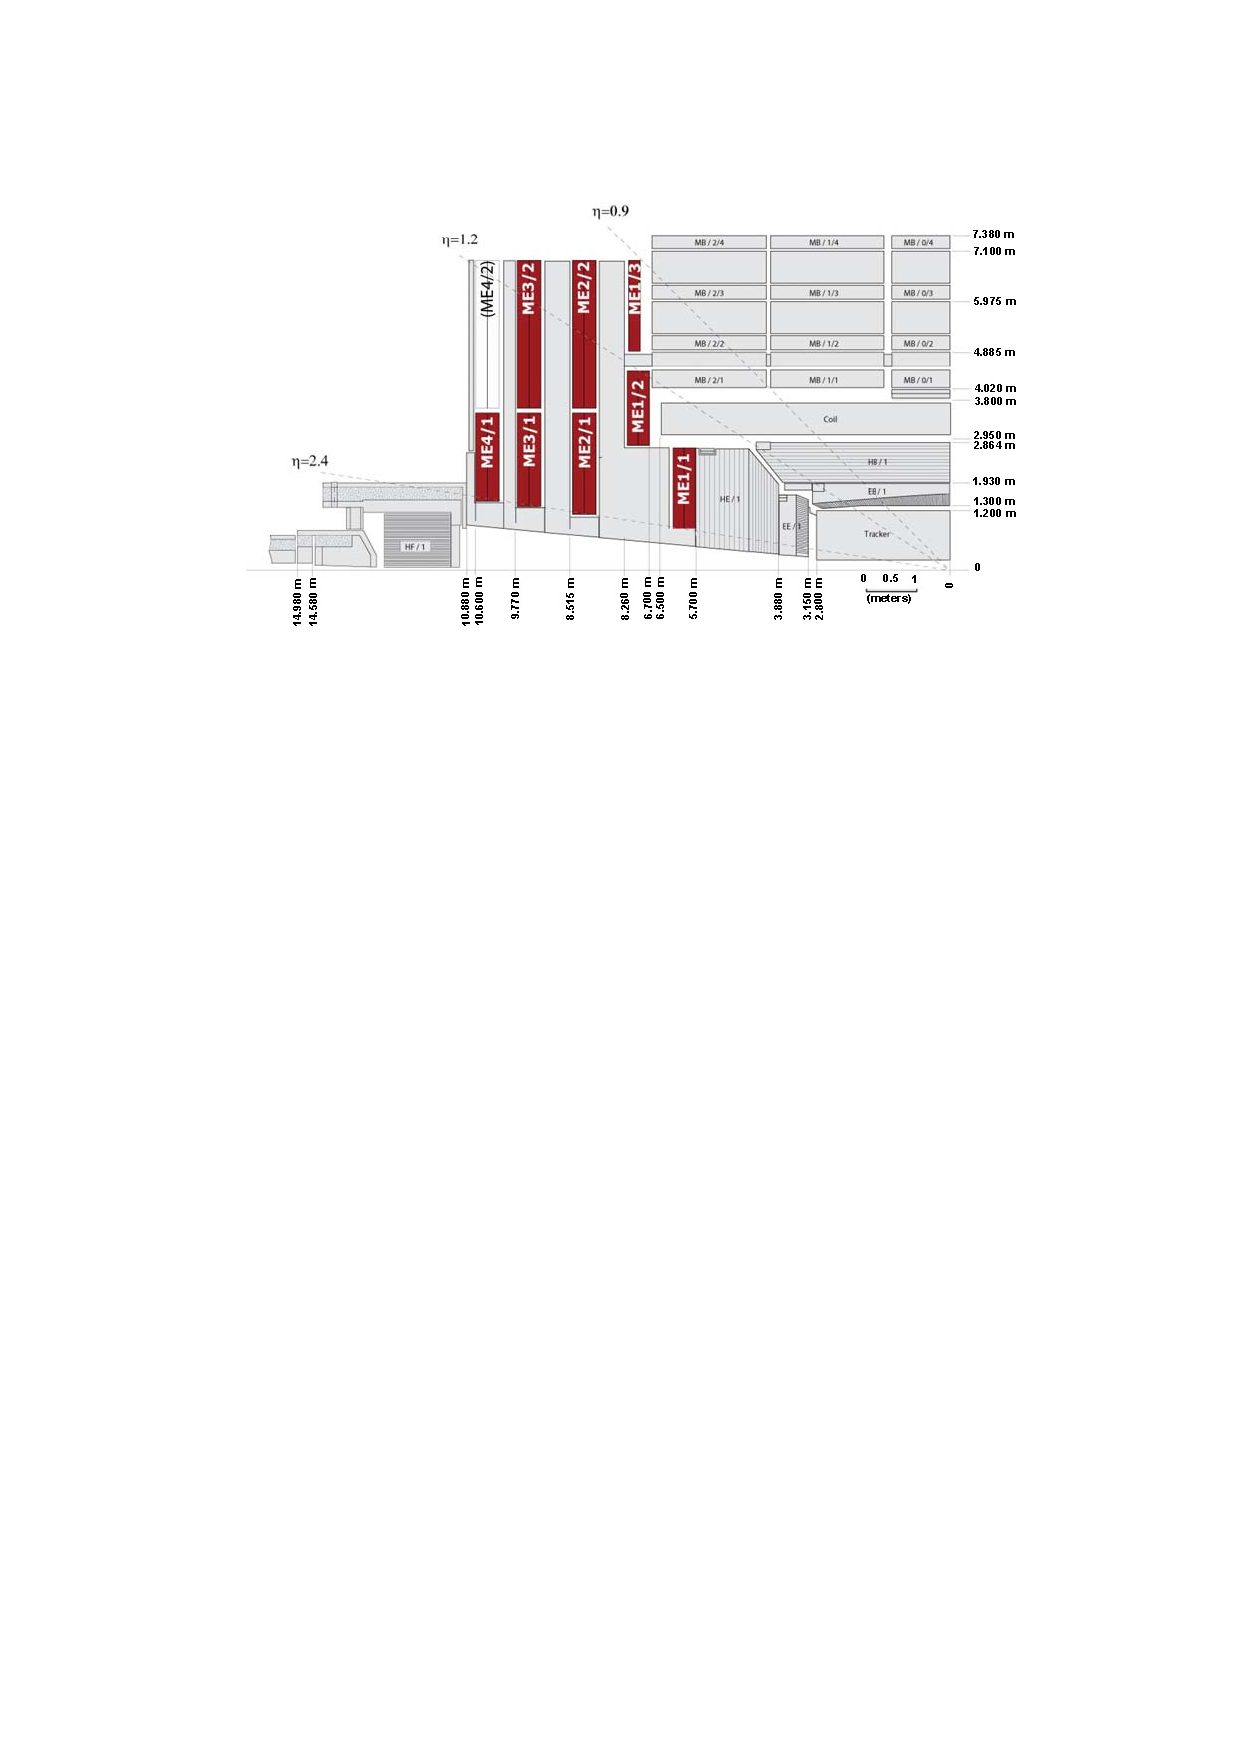
\includegraphics[width=4in]{figures/cscs.pdf}
\caption{Schematic diagram showing CSC locations in red in a quadrant cutout of CMS \cite{1748-0221-3-08-S08004}.}
\label{fig:cscs}
\end{figure}

The final muon subsystem, the 480 rectangular barrel and trapezoidal end cap RPCs, are arranged in six barrel layers, two in stations one and two, and one each in stations three and four, and in three layers in each end cap. The RPC modules contain parallel-plate detectors with $2-3$ double-gap modules of up to 96 (32) strips, parallel (radial) to the beam line in the barrel (end cap) sections, which collect ionized charge carriers from the 96.2\%:3.5\%:0.3\%, $\rm{C}_2\rm{H}_2\rm{F}_4$:$\rm{C}_4\rm{H}_{10}$:S$\rm{F}_6$ gas. A schematic of the module layout is shown in Figure~\ref{fig:rpcs}. The timescale in which RPCs can tag events is faster than the 25 ns bunch crossing time of the LHC, which in combination with the other muon systems, allows efficient triggering on muon events, discussed further in the next section.

\begin{figure}[tbh]
\centering
\begin{subfigure}{0.45\textwidth}
\centering
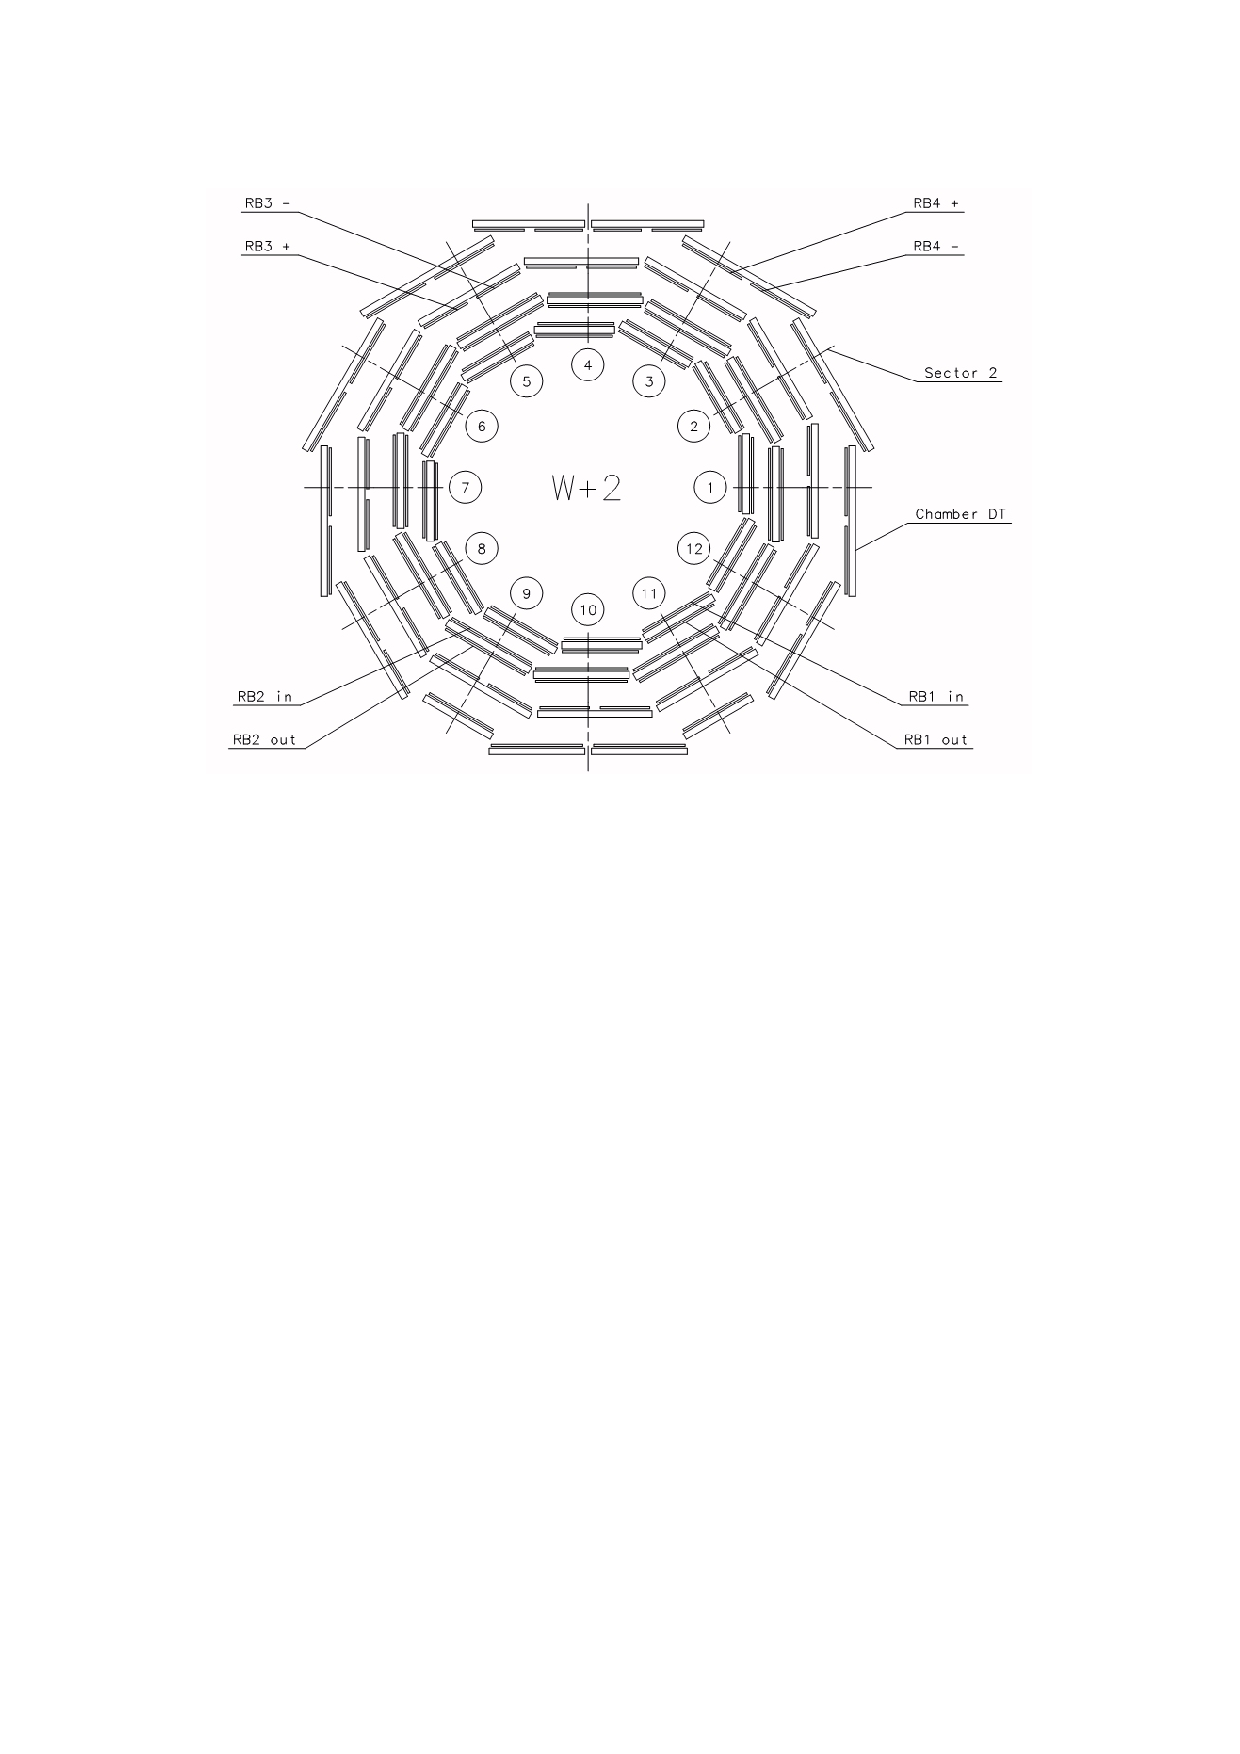
\includegraphics[width=3in]{figures/rpcbarrel.pdf}
\caption{}
\end{subfigure}
\begin{subfigure}{0.45\textwidth}
\centering
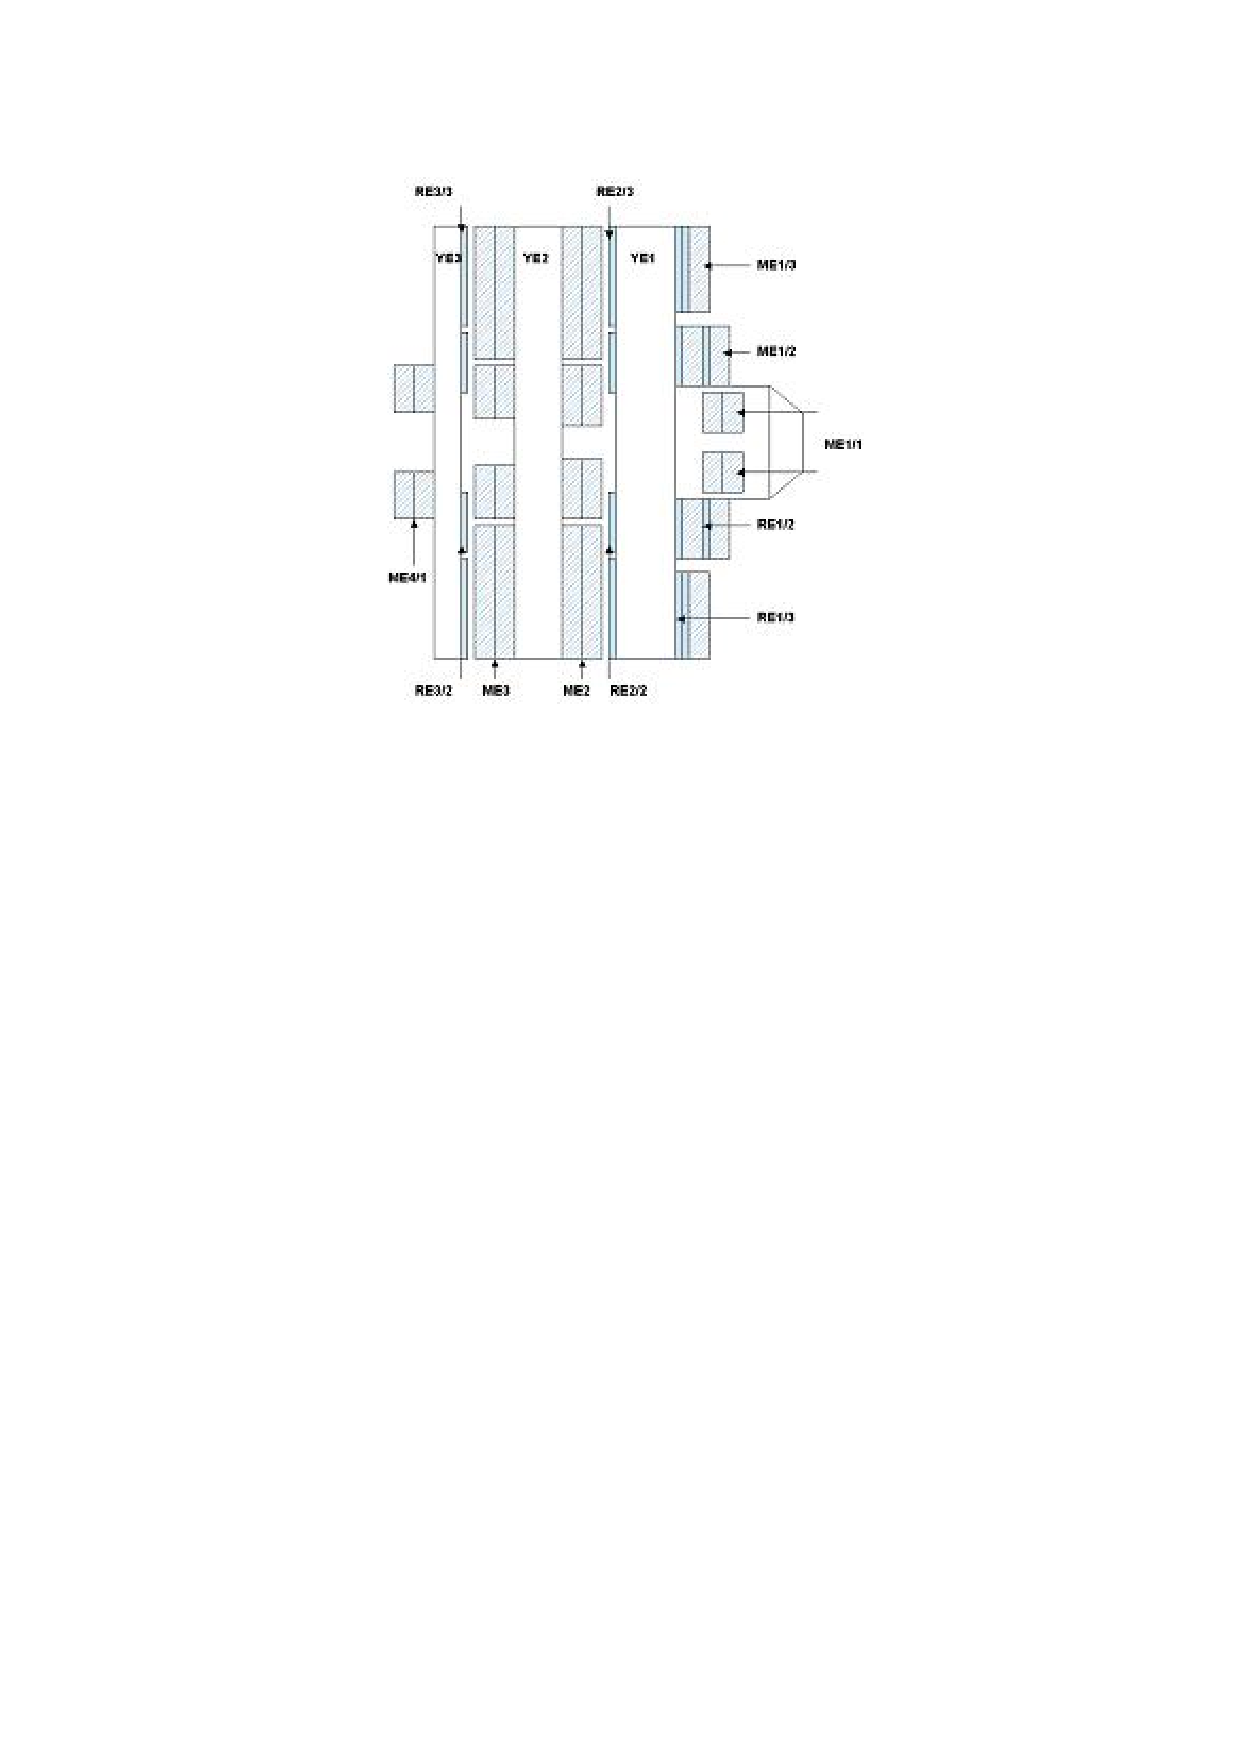
\includegraphics[width=3in]{figures/rpcendcap.pdf}
\caption{}
\end{subfigure}
\caption{Schematic diagram showing barrel RPC locations (left) and end cap RPCs (right) in a cross sectional cutout of CMS \cite{1748-0221-3-08-S08004}.}
\label{fig:rpcs}
\end{figure}

\indent The objective of the muon system to accurately measure the momenta of muons over a wide pseudorapidity range is accomplished, as shown by the less than 6\% transverse momentum resolution shown in Figure~\ref{fig:muonres} \cite{1748-0221-7-10-P10002}.

\begin{figure}[tbh]
\centering
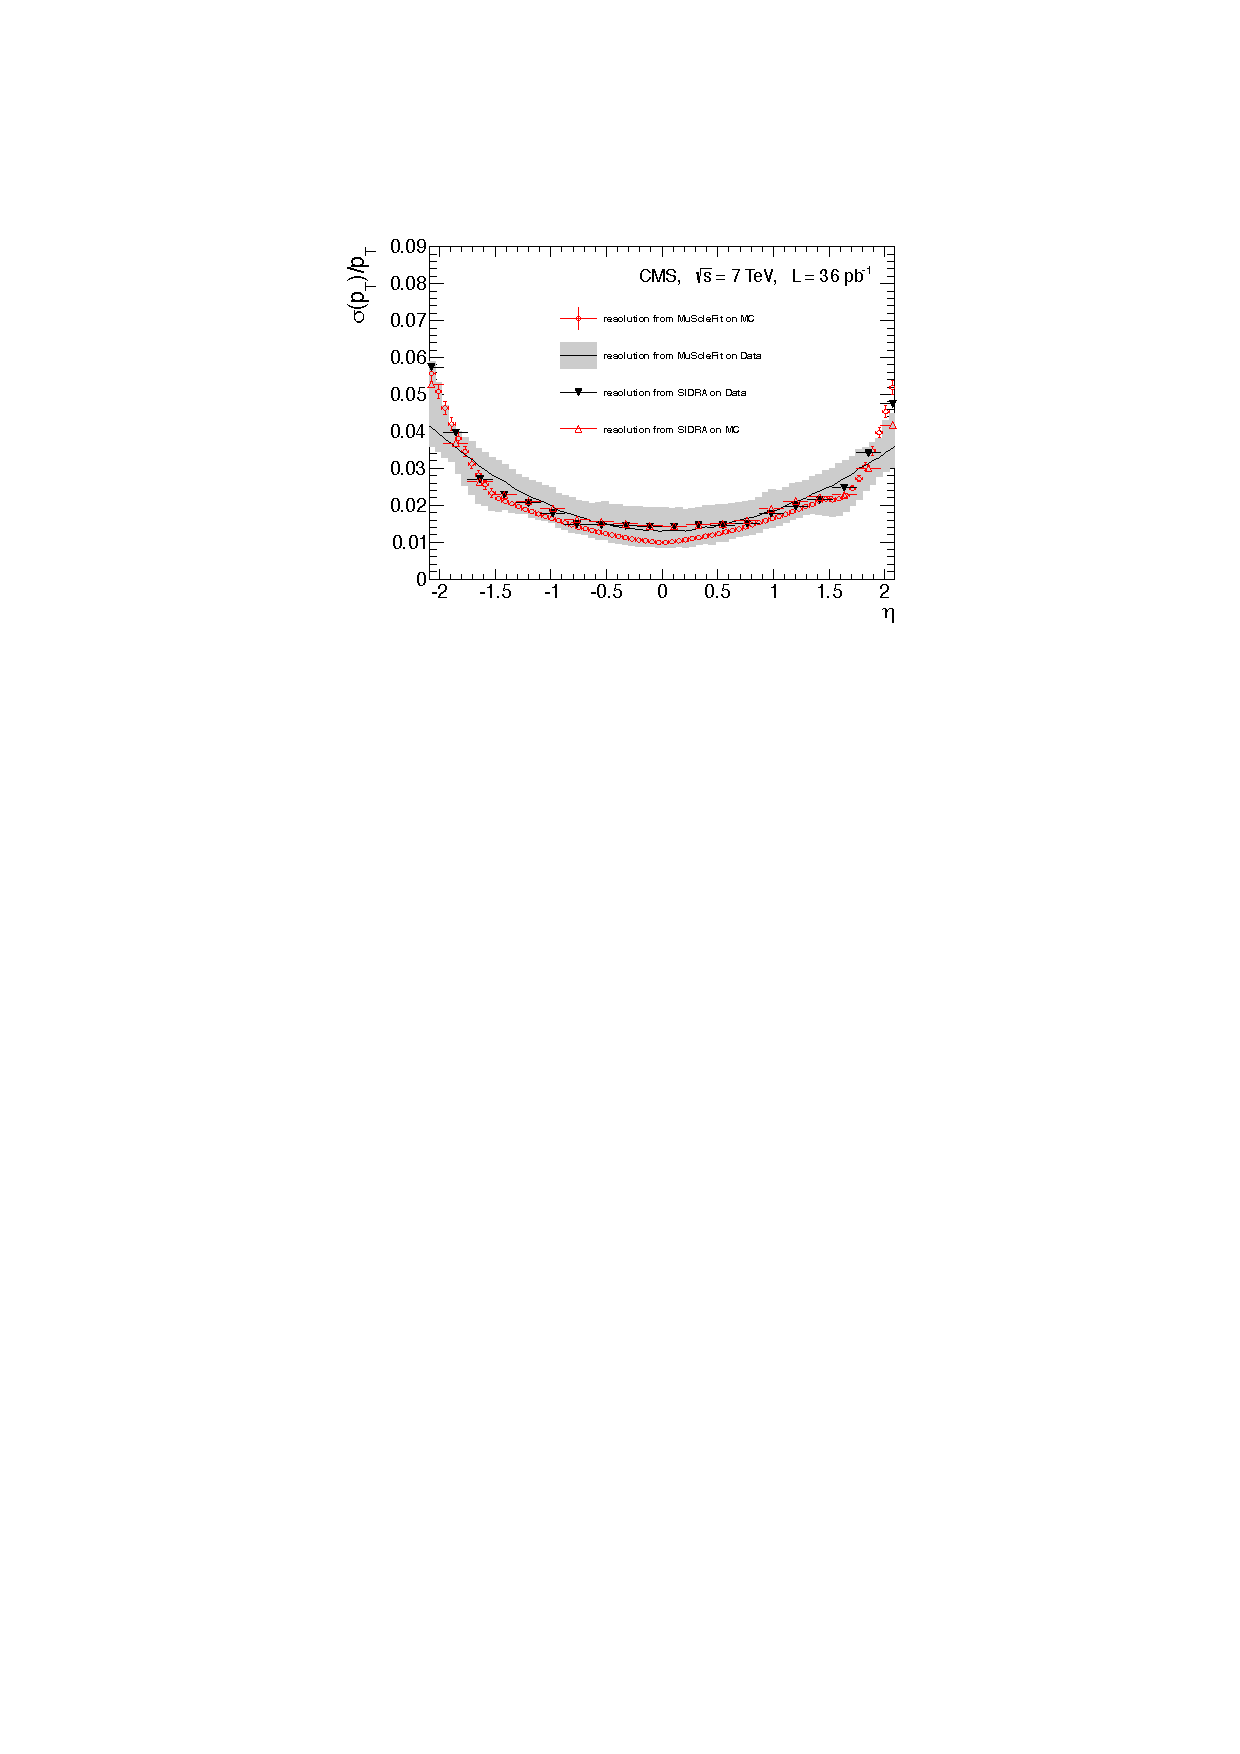
\includegraphics[width=5in]{figures/muonres.pdf}
\caption{Transverse momentum resolution versus pseudorapidity for muons from $Z$ decays \cite{1748-0221-7-10-P10002}.}
\label{fig:muonres}
\end{figure}

\subsection{Trigger}

In order to reduce the O(100) MHz interaction rate from LHC proton collisions to a computationally manageable O(100) kHz rate, a trigger system consisting of an Level-1 Trigger (L1T) and a High-Level Trigger (HLT) is employed. The L1T, summarized in Figure~\ref{fig:l1t}, uses mainly field programmable gate array (FPGA) technology on the front-end electronics to compile local trigger primitives from calorimeter towers and muon tracks into regional triggers, which use pattern logic to identify objects like electrons and muons. The highest quality objects are piped to the global trigger, which decides, based on further calculations and input on the status of the subdetectors, whether an event is rejected or an L1 Accept signal is sent to the Timing, Trigger, and Control (TTC) system for reading out the front-end data buffers, with a latency of 3.2 $\mu$s.

\begin{figure}[tbh]
\centering
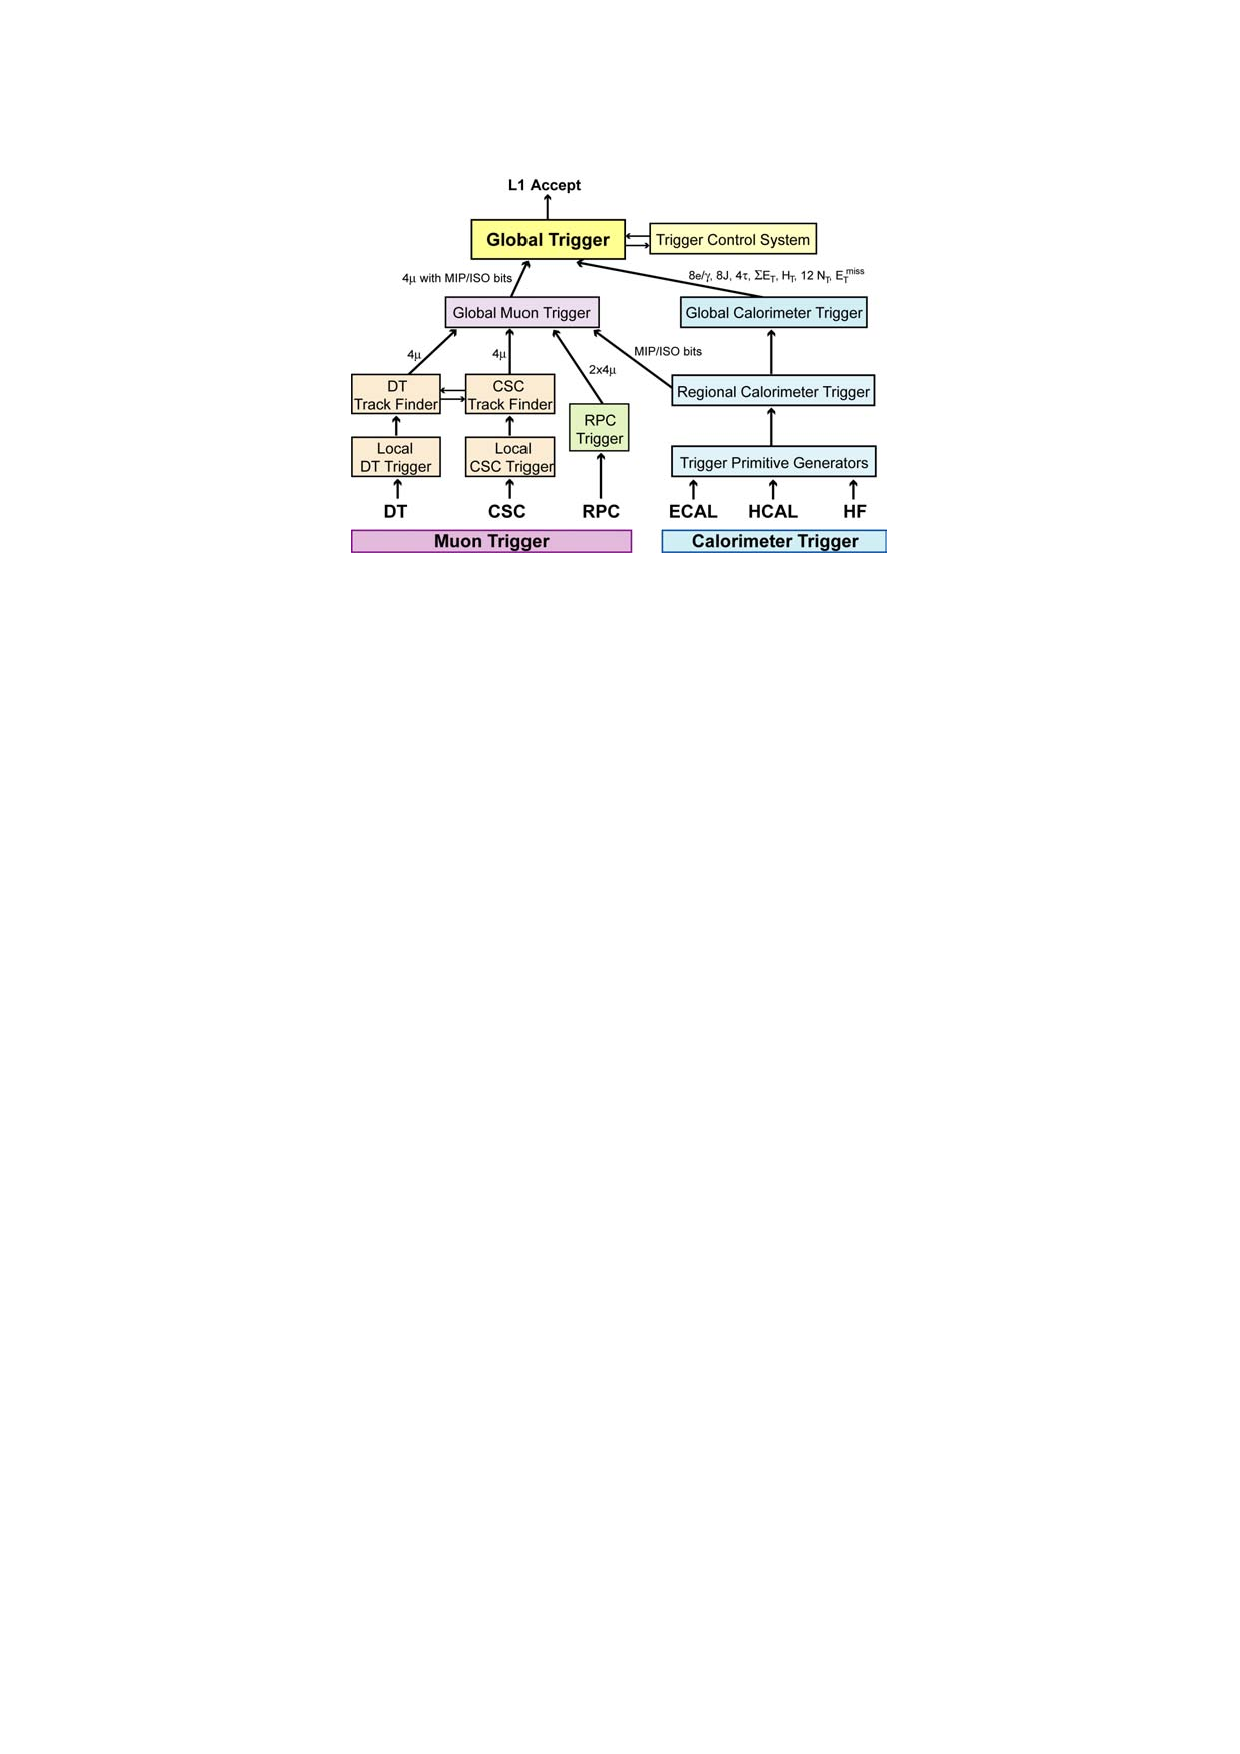
\includegraphics[width=5in]{figures/l1t.pdf}
\caption{CMS L1 trigger system schematic diagram \cite{1748-0221-3-08-S08004}.}
\label{fig:l1t}
\end{figure}

\indent After an event passes the L1T, the entire event data is read out by the data acquisition (DAQ) system, summarized in Figure~\ref{fig:daq}. First, data is read out from the subdetector front-end buffers to the front-end drivers (FEDs), followed by the merging of FED fragments by the Event Builder and the submission of the complete event data to the HLT by the Event Filter. The HLT is a software system, which uses filtering and reconstruction algorithms to select events based on their physics object content, with different paths based on the different combinations of objects used in physics analyses. The HLT paths used in this analysis are based on combinations of high quality lepton objects, such as two muons or two electrons, and are discussed further in the next chapter. Data quality monitoring (DQM), is also carried out at this step, to ensure all subsystems are behaving properly and the data being collected is usable for analysis. Data passing the HLT is saved to storage and processed in the offline software system before being provided to analyzers for physics searches. 

\begin{figure}[tbh]
\centering
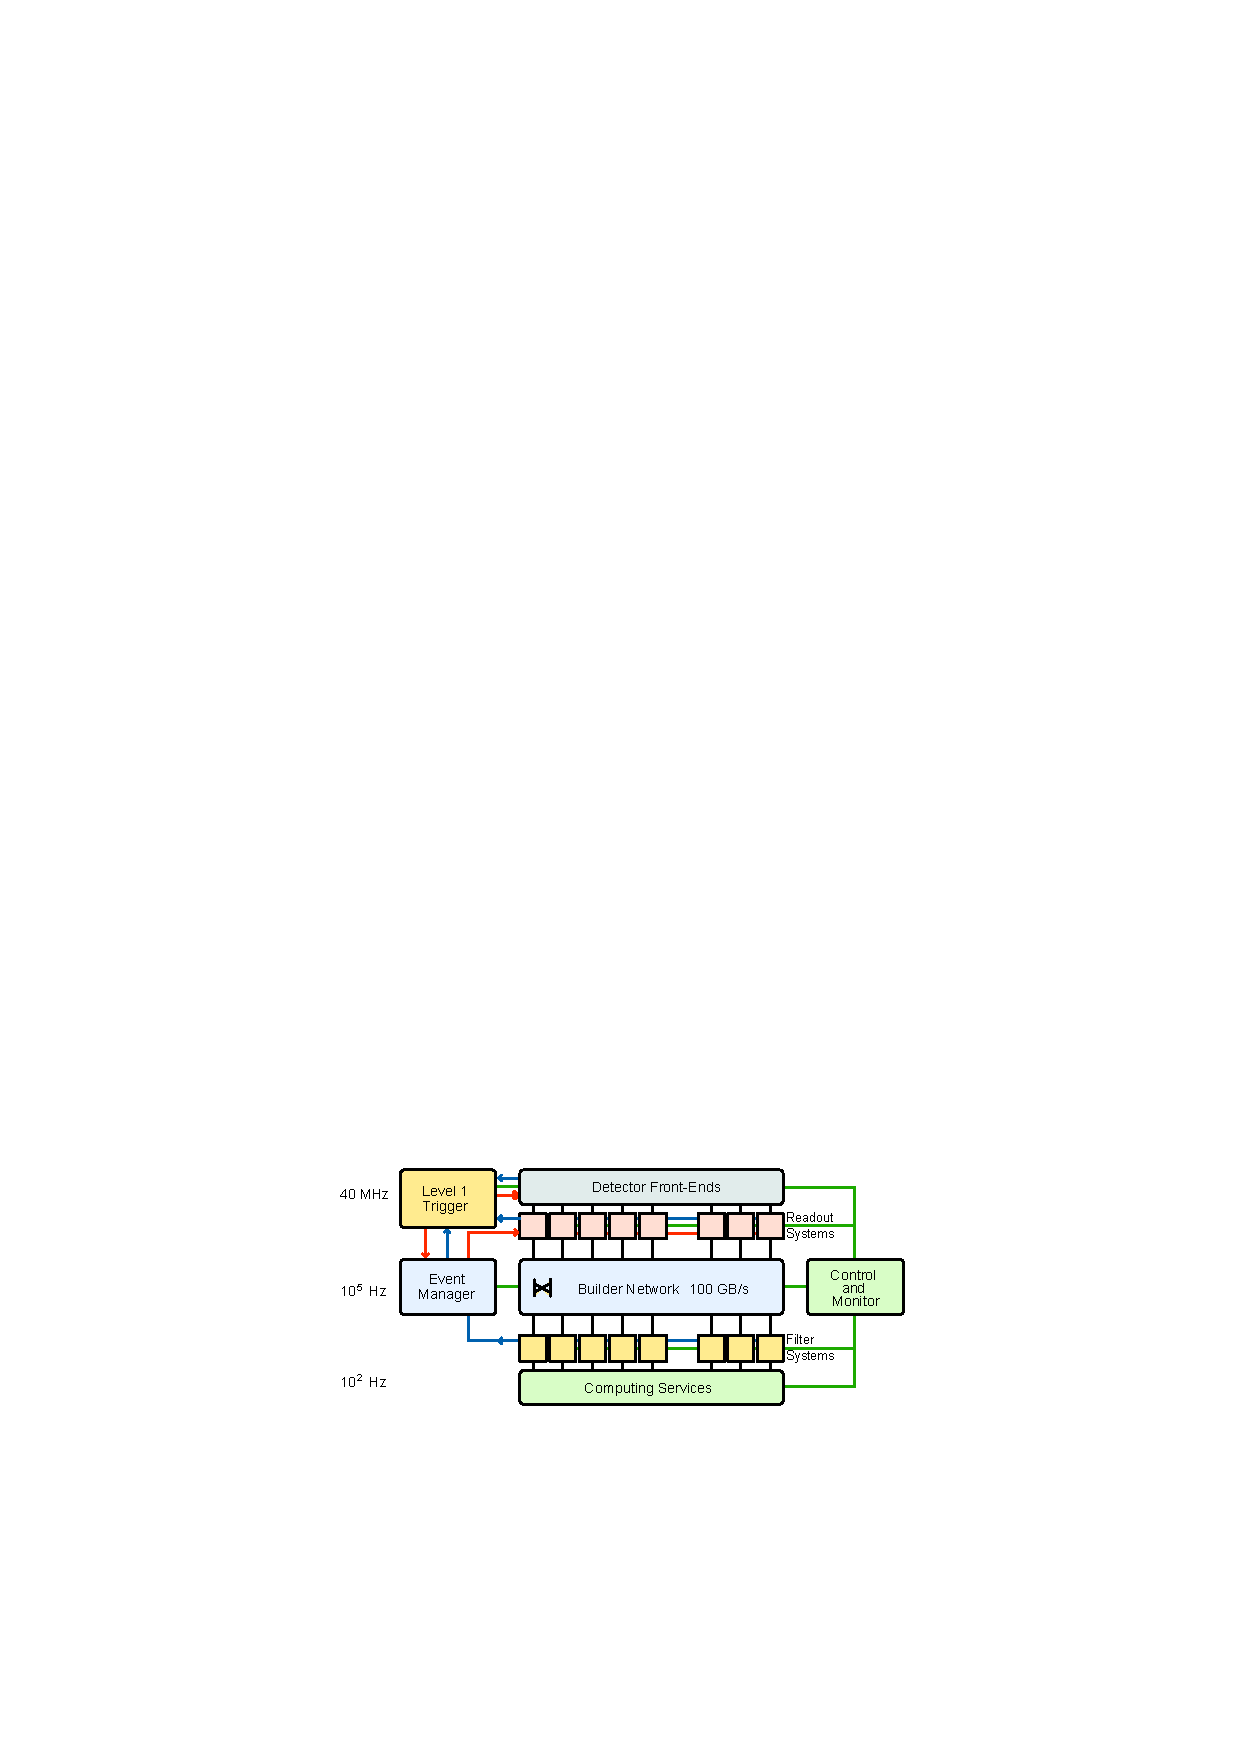
\includegraphics[width=5.5in]{figures/daq.pdf}
\caption{CMS data acquisition system schematic diagram \cite{1748-0221-3-08-S08004}.}
\label{fig:daq}
\end{figure}

\indent In order to verify that the live trigger system is performing as expected and to emulate the trigger system for the production of simulated events, an offline trigger software framework is developed and maintained in parallel with the hardware system. For each calorimeter and muon trigger subsystem, there is a corresponding software emulator that simulates the hardware decisions. The live DQM system used by trigger shifters compares the hardware output to the output of the emulators. In addition to DQM, the trigger software framework is used to calculate the L1T efficiencies, or the efficiency of detection for various reconstructed physics objects. The service work conducted in the process of completing this thesis included contributing to the upgrade of the offline software to be based on calorimeter Layers instead of the regional (RCT) and global trigger (GCT) subsystems of the Run 1 legacy format described above, and the development of automated workflows for trigger DQM. The Run 2 calorimeter trigger system is based on two layers: Layer1, responsible for constructing towers from the energy deposits in ECAL and HCAL modules, and Layer2, which algorithmically builds physics objects from Layer1 towers. A staggered upgrade plan was carried out with the GCT replaced by Layer2 in 2015 (called Stage1) and the RCT to Layer1 in 2016 (called Stage2). During partial upgrades, data formats would be upconverted or downconverted before or after an upgrade stage, where applicable, to keep the entire workflow functioning. 

